% !TEX encoding = UTF-8 Unicode

% PACKAGES 

\documentclass[a4paper,11pt, twoside, openright]{book}

\usepackage[english]{babel}
\usepackage[T1]{fontenc}
\usepackage{amssymb}
\usepackage{amsmath}
\usepackage[hyphens]{url}
\usepackage{cite}
\usepackage{graphicx}
\usepackage[utf8]{inputenc}
\usepackage{enumitem}
\usepackage{float}
\usepackage{framed}
\usepackage{pseudocode}
\usepackage{listings}
\usepackage{courier}
\usepackage{rotating} 
\usepackage{color}
\usepackage{colortbl} 
\usepackage{xcolor}
\usepackage[times]{quotchap}
\usepackage{caption}
\usepackage{subcaption}
\usepackage{textcomp}
\usepackage{perpage}
\usepackage{fancyhdr}
\usepackage{pifont}
\usepackage{calc}
\usepackage{nameref}
\usepackage[ % ---- FILL IN THE DOC TITLE AND AUTHOR
	bookmarks,
	colorlinks, 
	breaklinks, 
	pdftitle={Fixing The Web},
	pdfauthor={Roeland Matthijssens},
]{hyperref}
\usepackage{cleveref}
\usepackage{sty/chapterimages}
\usepackage{siunitx}

% FONTS
\newcommand{\amper}{{\fontspec[Scale=.95]{Gentium Basic Italic}\selectfont\itshape\&}}
\newcommand{\kopiraajt}{{\fontspec[Scale=.95]{Gentium Basic Italic}\selectfont\itshape\copyright}}

% COMMANDS

\newcommand{\todo}[1]{\textcolor{red}{[TODO: #1]}}
\newcommand{\dquote}[1]{``#1''}
\newcommand{\squote}[1]{`#1'}
\newcommand{\code}[1]{\texttt{#1}}
\newcommand{\speech}[1]{\emph{\dquote{#1}}}
\newenvironment{requirements}{\begin{framed} \textbf{Requirements}}{\end{framed}}
\newcommand{\xmark}{\ding{55}}
\newcommand{\cmark}{\ding{51}}

% SETTINGS

\raggedbottom
\graphicspath{{images/}}
\numberwithin{figure}{chapter}
\renewcommand{\thefigure}{\thechapter-\arabic{figure}}
\renewcommand{\thetable}{\thechapter-\arabic{table}}
\MakePerPage{footnote}
\PassOptionsToPackage{usenames}{color}
\hypersetup{
	breaklinks=true,
 	colorlinks=true,
	linkcolor=black,
	citecolor=blue,
	filecolor=black,
	urlcolor=blue,
	pdfborder={0 0 0},
	pdfcreator = {LaTeX},
  	pdfproducer = {pdfLaTeX},
  	bookmarksopen=true
}
\renewcommand{\lstlistlistingname}{List of Listings}
\setcounter{secnumdepth}{3}
\renewcommand*{\chapterautorefname}{Chapter}
\crefname{figure}{Figure}{Figures}
\renewcommand*\arraystretch{1.9}

% LISTINGS

\definecolor{darkgreen}{rgb}{0,0.6,0}
\definecolor{blue}{rgb}{0,0,1}
\definecolor{lightgray}{rgb}{0.9,0.9,0.9}
\definecolor{darkgray}{rgb}{.4,.4,.4}
\definecolor{purple}{rgb}{0.65, 0.12, 0.82}
\definecolor{gray}{rgb}{0.4,0.4,0.4}
\definecolor{darkblue}{rgb}{0.0,0.0,0.6}
\definecolor{cyan}{rgb}{0.0,0.6,0.6}

\lstdefinelanguage{JavaScript}{
  keywords={typeof, new, true, false, catch, function, return, null, catch, switch, var, if, in, while, do, else, case, break},
  keywordstyle=\color{blue}\bfseries,
  ndkeywords={class, export, boolean, throw, implements, import, this},
  ndkeywordstyle=\color{darkgray}\bfseries,
  identifierstyle=\color{black},
  sensitive=false,
  comment=[l]{//},
  morecomment=[s]{/*}{*/},
  commentstyle=\color{purple}\ttfamily,
  stringstyle=\color{red}\ttfamily,
  morestring=[b]',
  morestring=[b]"
}

\lstset{
 language=JavaScript,
  backgroundcolor=\color{lightgray},
  extendedchars=true,
  basicstyle=\footnotesize\ttfamily,
 showstringspaces=false,
 showspaces=false,
 numbers=left,
 numberstyle=\footnotesize,
  numbersep=9pt,
  tabsize=2,
  breaklines=true,
  showtabs=false,
 captionpos=b,
  frame=single,
  frameround=tttt,
}

\lstdefinelanguage{XML}
{
  morestring=[b]",
  morestring=[s]{>}{<},
  morecomment=[s]{"}{"},
  stringstyle=\color{black},
  identifierstyle=\color{darkblue}\bfseries,
  commentstyle=\color{darkgreen},
  keywordstyle=\color{darkblue},
  morekeywords={xmlns,version,type,theme,source,name,ref,minOccurs,maxOccurs,mixed,src,default,data,author,rel,id,x,y,rotate,title,layout,href,duration,start,position}% list your attributes here
}

\lstdefinelanguage{Hack1}
{
  morestring=[b]",
  morestring=[s]{>}{<},
  morecomment=[s]{"}{"},
  stringstyle=\color{black},
  identifierstyle=\color{darkblue}\bfseries,
  commentstyle=\color{darkgreen},
  keywordstyle=\color{darkblue},
  morekeywords={xmlns,version,type,theme,source,ref,minOccurs,maxOccurs,mixed,src,default,data,author,rel,id,x,y,rotate,layout,href}% list your attributes here
}

\hyphenation{tech-no-lo-gy}

% TITLE PAGE SETTINGS

\usepackage{sty/vub}

\author{Roeland Matthijssens}
\title{Fixing The Web: }
\extendedtitle{Combining Advanced Linking and Visualisation in HTML5 based on RSL}
\subtitle{Proefschrift ingediend met het oog op het behalen van de titel Master of Science in de Toegepaste Informatica, door:}
\faculty{FACULTEIT WETENSCHAPPEN EN BIO-INGENIEURSWETENSCHAPPEN}
\department{Departement Computersience \newline Web \& Information Systems Engineering Laboratory}
\promotortitle{Promotor}
\advisortitle{Begeleider}
\promotor{Prof. Dr. Beat Signer}
\advisors{Prof. Dr. Beat Signer}
\date{Augustus 2013}
\selectlanguage{english}


% PAGE HEADER AND FOOTER

\begin{document}

\pagestyle{fancy}
\setlength{\headheight}{14pt}
\renewcommand{\chaptermark}[1]{\markboth{\MakeUppercase{\chaptername}\ \thechapter.\ #1}{}}
\renewcommand{\sectionmark}[1]{\markright{#1}{}}
\fancyhf{}
\fancyhead[LO,RE]{\bfseries\thepage}
\fancyhead[RO]{\bfseries\leftmark}
\fancyhead[LE]{\bfseries\rightmark}
\renewcommand{\headrulewidth}{0pt}

% PARAGRAPH INDENTATION

\setlength{\parskip}{0pt} % 1ex plus 0.5ex minus 0.2ex}
\setlength{\parindent}{0pt}

%
% TITLE PAGES
%

\pagenumbering{alph} % required so there are no conflicting page numbers

\vubtheses

\pagebreak

\thispagestyle{empty}
\vspace*{\fill}
\begin{center}
\copyright Vrije Universiteit Brussel, all rights reserved.
\end{center}

\pagebreak

\subtitle{Graduation thesis submitted in partial fulfillment of the requirements for the degree of \newline Master in Applied Computer Science, by: }
\faculty{FACULTY OF SCIENCE AND BIO-ENGINEERING SCIENCES}
\department{Department of Computer Science \newline Web \& Information Systems Engineering Laboratory}
\promotortitle{Promoter}
\advisortitle{Advisor}
\promotor{Prof. Dr. Beat Signer}
\advisors{Prof. Dr. Beat Signer}
\date{August 2013}

\vubthesesen

\pagebreak

\thispagestyle{empty}
\vspace*{\fill}
\begin{center}
\copyright Vrije Universiteit Brussel, all rights reserved.
\end{center}

\pagebreak


\makeatletter\@openrightfalse

%
% ABSTRACT
%
\pagestyle{empty}
\pagebreak
\newpage
%!TEX root = thesis.tex 

\chapter*{Abstract}
\thispagestyle{empty}
\paragraph{}
With over \num{150000} new websites being produced every day, the World Wide Web is playing an increasingly more important role in day to day life. From personal use to big Internet companies, the Web is omnipresent in a modern society. The Web was created in the late 1980s and has been publicly available since 1991. However, after all this time, very little has changed to the core ideas. The idea of the Web was seeded by Vannevar Bush's vision of the Memex but has evolved hastily to match the needs of the consumers. This haphazard evolution of the Web gave priority to new flashy features neglecting the foundation of the Web: Linking different resources together. Modern websites are still mostly using simple anchor tags, a technique designed in 1994, to link their web pages together.
\paragraph{}
In this thesis, we take a critical stance toward conventional linking techniques and the popular tools that have become a standard for browsing the Web. From an evolutionary point of view, it is clear why the current standard includes outdated techniques. Even though anchor tags are the single most used technique to link resources together, it does not imply that this is the most optimal or complete approach.
\paragraph{}
Through literature study and critical thinking, we identify a number of important flaws and shortcomings regarding the core concepts of standard linking techniques on the Web. A closer look at alternative approaches showed that more advanced and complete approaches are already available. By studying these alternatives and taking a step back from the dogma of standard linking techniques, we were able to apply state-of-the-art research from the fields of information management and visualisation, effectively increasing the Web's potential and ameliorating the majority of its current limitations. Our proposed solution provides a new angle on the way resources can be linked on the Web and bases itself on recent research in the areas of hypermedia and data visualisation.
\paragraph{}
Separating the linking metadata from the structure of the web page minimises the misapplication of markup languages which are currently used to link different resources together. This separation will pave the way for more complex linking structures which will in turn provide increased functionality on the Web. The increased functionality allows users to share their metadata with each other which is currently a dominant evolution on the Web. User communities will fill large databases with associative links between different web resources, sharing their knowledge and insights. In time the amount of metadata that is generated will be of such large proportions that adding all this additional data to a web page will make it unusable and unreadable. We combine the research from the field of data management and the findings from our literature study to propose a scalable solution to these newly introduces issues. Our solution also separates the visualisation of the metadata from the web page allowing us to employ innovative techniques from the fields of data visualisation and interactive user interfaces. Furthermore, the use of the latest HTML5 standards for the visualisation and JavaScript for the implementation ensures minimum coupling with maximum compatibility.
\paragraph{}
While it is perfectly possible to create classic hyperlinks with our solution, it offers features that go beyond state-of-the-art linking techniques. Our solution provides the means to step away from the unidirectional single source and single target hyperlinks that traditional linking solutions provide. The choice of technology allows a degree of interactivity that is impossible with existing tools providing interactive filtering, navigation and searching as well as many other features that are unheard of in current state-of-the-art linking solutions.



%Through our innovative MindXpres solu-
%tion, we are going to enhance the presentation experience for the presenter
%and audience alike in the near future!
\newpage

\@openrighttrue\makeatother
%
% ACKNOWLEDGEMENTS
%
\chapter*{Acknowledgements}
\paragraph{}
First of all, I would like to thank my promoter and advisor, Prof.~Dr.~Beat Signer for giving me the opportunity to research this topic and for his invaluable support. I would like to express my deepest gratitude for the endless patience and countless hours you spend proof-reading every detail of this document.
\paragraph{}
My special thanks goes out to Rik Vanmechelen, Reinout Roels and Ruben Tytgat, whom I count as dear friends. I honestly feel I would not have made it this far without their constant support and rubber ducking when I needed it most.

\paragraph{}
I would like to thank Riot, Valve and Firaxis for helping me keep my sanity during the more difficult periods of the project.

\paragraph{}
Most importantly, I would like to thank my girlfriend, Vanessa Gerrits for bearing with me through countless nights of working late. Her endless patience while reading and rereading all the drafts of this thesis were invaluable, as was her constant loving support.
\paragraph{}



%
% TABLE OF CONTENTS
%

\newpage
\pagestyle {fancy}
\pagenumbering{Roman}
\tableofcontents
\pagebreak
\thispagestyle{plain}

\makeatletter
\renewcommand*\cleardoublepage{\clearpage\if@twoside % chapter starts on odd pages
  \ifodd\c@page \hbox{}\newpage\if@twocolumn\hbox{}%
  \newpage\fi\fi\fi}
\makeatother

\pagenumbering{arabic}
\setcounter{page}{1}

%
% CONTENT
%

%!TEX root = thesis.tex 

\chapter{Introduction} \label{cha:Introduction}
\paragraph{} 
We are currently living in an information age where an estimated \num{150000} new websites are created on a daily basis. Since the HTML 2.0 standard was introduced in 1995, content creators are able to add anchor tags to their websites. These tags allow web pages to be interlinked, forming a vast web of information. To navigate this Web, we use browsers such as Google Chrome\footnote{\url{http://www.google.com/chrome/}}, Mozilla Firefox\footnote{\url{http://www.mozilla.org/firefox/}}, Safari\footnote{\url{http://www.apple.com/safari/}} or Oracle's Opera\footnote{\url{http://www.opera.com}}.

\paragraph{} 
The HTML standard has gone through several iterations since HTML 2.0. We are currently at HTML5 and a lot of features have been changed and added. However, the way web pages are linked together has remained unchanged. The main mechanism web developers use to create links between web pages is still the same anchor tag that was introduced almost 20 years ago. This anchor tag is not without limitations though and the only type of links that can be established using anchor tags are unidirectional single source and single destination links between two resources.

\paragraph{} 
 One possible definition for the Web that we could define is the following: \dquote{\emph{A system of interlinked hypertext documents accessed via the Internet}}. The core of this definition is that these pages need to be interlinked, therefore it is rather strange that the technology that is used to create these links has not been updated or improved over the last decades.

\paragraph{} 
HTML and HTTP were invented in 1990 by Sir Timothy John Berners-Lee~\cite{fielding1998hypertext}. The term hypertext was already coined in 1965 by Ted Nelson~\cite{myers1998brief}, predating the HTML standard by a couple of decades. Nelson defines hypertext as \dquote{\emph{Non-sequential writing}} meaning that the text can branch in different directions. At a certain point in a block of text, a pointer may be introduced that directs the readers to a different section, or even a different document. Ted Nelson's idea of hypertext was heavily influenced by Vannevar Bush and his idea of the Memex~\cite{Bush1945As}. With his hypertext, Nelson aims to mimic the associative links between content as introduced by Bush. Ted Nelson's hypertext idea may sound reminiscent of the current HTML's anchor tags, where one source can embed a link to another source. But in fact Ted Nelson stated that his vision of hypertext actually tried to prevent the evolution that is currently active in HTML standards~\cite{nelson1987computer}. HTML only supports unidirectional links, and as a result, quotes cannot be followed back to their original source. There is also no notion of version or rights management and existing links keep breaking when the content of websites is updated. Nelson stated, that due to these limitations the current HTML standard is a major oversimplification of his original idea of hypertext and hypermedia\footnote{\url{http://hyperland.com/TedCompOneLiners}}.

\paragraph{} 
These obvious problems with linking in HTML were the cause of several initiatives attempting to \dquote{fix the web} and get closer to the initial ideas of hypertext and hypermedia. Most of these initiatives originate from other research labs that aim to enhance the Web. The main difference between existing tools and our tool is the setting in which it will be used. Existing tools were designed and developed as a private tool to be used by a single person for their own personal interests. At best, these tools could be used by small groups of users sharing the same interests and needs. The solution we will present in this thesis is designed and developed as a tool for communities or even large sets of different communities with different interests and needs. However, in designing this tool, we encountered an important problem. This problem was less obvious in existing tools because they were intended to be used by a single person which, in most cases, greatly limits the amount of data the tool would have to operate on. When we increased the amount of users that will use the tool simultaneously, we encountered some interesting issues.

\paragraph{} 
Imagine users annotating a web page with comments and adding a links between two web pages they have previously visited. Users will highlight sentences or words on these pages to mark the location of the annotation and the sources of the links. Because they are the only users using the system, they can choose to not create too many hyperlinks on a specific paragraph to keep the content readable. They will also adopt a specific scheme of annotating that will suit their work style and keep the web pages usable. In other words, the user can easily control the amount of metadata that is put on a specific page. If a page gets too cluttered for the users' taste, they can remove or rewrite some of the annotations until the web page is to their liking once more. In a multi-user setting, this issue becomes a lot more prominent. Imagine a popular news website that gets thousands of daily hits. A good percentage of these users will read an article about something they have read before. These users will share their information with the rest of the community by adding an annotation to the article or by adding a link to another website that has more information on the topic. Since there are thousands of users reading this specific article, it is possible that too many users try to share their information, thus quickly cluttering the text with metadata. If we naively add all this extra data to the web page the page will become unreadable and the tool will hinder the users instead of helping them find additional information. For most of the existing tools, the usability of the tool is therefore inversely proportional to the amount of users that will share their data with each other.

\paragraph{} 
The main problem when a multitude of users are sharing the same database is actually a visualisation problem. The usability issues that other tools have, originate from their naive way of visualising the metadata on the web page. The question that arises is the following: \dquote{\emph{How can we make use of the metadata that is generated by a large community of users, without reducing the usability of the web page?}} To answer this question we need to explore several different aspects of the problem.
\begin{itemize}
	\item \textit{Filtering} How can we distil the important and relevant data out of the vast amounts of generated metadata in order to help users find what they are looking for more quickly?
	\item \textit{Visualising} How will we visualise the selected metadata in such a way that the users have a clear overview of the available information without making the web page unreadable?
	\item \textit{Interaction} With techniques to create more complex hyperlinks with multiple destinations and multiple sources we need to provide more powerful interactions for the users to browse this more complex Web.
\end{itemize}

\paragraph{} 
In this thesis we explore previous attempts to increase the Web's linking functionality and investigate areas where improvements can be made. In Chapter \ref{cha:Limitations of Linking Techniques}, we discuss the current techniques that are used to link resources. We proceed by showing why these techniques are suboptimal and why there is a need for improved linking functionality. In Chapter \ref{cha:Towards a Better Web}, we take a look at alternative approaches to the default HTML linking. These alternative tools give us additional insights on how we could improve upon the default linking functionality.

\paragraph{} 
Based on our conclusions from Chapter \ref{cha:Towards a Better Web} and combined with our personal insights, we define the key concepts that our tool needs to provide in Chapter~\ref{cha:An Alternative Approach}. By generalising our problem to a data visualisation problem instead of limiting us to the canvas of a web page, we can apply recent work in the active field of data visualisation. These insights help us to mitigate some of the problems alternative approaches introduced. In Chapter \ref{cha:The Tool}, we propose a different solution based on our findings in Chapter \ref{cha:An Alternative Approach}. This solution is then implemented and discussed in Chapter \ref{cha:Implementation}. In order to demonstrate the benefits that our solution claims to provide, we follow up the implementation with use cases that will show how the tool operates in a real world setting. This is done in Chapter \ref{cha:Use Cases} where we walk through the entire process of authoring and navigating through annotations and hyperlinks, discussing our improvements along the way.

\paragraph{} 
As this is a Master's thesis, time was limited and our work is restricted by the available time. However, in Chapter \ref{cha:Conclusions and Future Work} we provide our conclusions as well as a discussionof some possible future work that could be carried out to further extend the tool.

\paragraph{} 
By extending the Web's current linking technology and by allowing communities to use a single database to share their metadata, we aim to provide a better web experience for both content creators and consumers. We are confident that our proposed tool improves many of the issues we have identified and greatly improves the accessibility of metadata for large groups of users.

%!TEX root = thesis.tex

\chapter{Limitations of Current Linking Techniques} \label{cha:Limitations of Linking Techniques}
	\paragraph{}
	In this chapter we take a closer look at the shortcomings of the standard HTML linking techniques. We point out why these shortcomings have a serious negative effect on the potential of the World Wide Web. We also elaborate on the reasons why these techniques became the standard way of linking, as well as why these techniques have not been updated over the last couple of decades.

%HISTORY {{{
\section{The History of The Web} \label{sec:The History Of The Web}
	\paragraph{}
	In 1980 Tim Berners-Lee was hired as an independent contractor for CERN where he was working on ENQUIRE\cite{caygill1999meno}, a personal database of people and software models. ENQUIRE was a simple hypertext program that had the same basic ideas of the World Wide Web and is therefore often referred to as its predecessor. However, many years before Tim Berners-Lee's work on what eventually became the World Wide Web, an American science-fiction writer named Murray Leinster wrote \dquote{A Logic Named Joe}, a short story published in 1946. The story describes the concept of a home-based global information system that had many of the same characteristics as the current Web.
	\paragraph{}
	In 1984 Tim Berners-Lee noticed a problem with CERN's information presentation. Physicists from all over the world needed to share their research with each other, but the lack of common machines and presentation software made this a cumbersome task. Therefore in 1989 he wrote a proposal for a large interlinked hypertext database~\cite{berners1989information}, but at the time this generated little interest. His boss Mike Sendalli however, believed in his ideas and encouraged him to start developing his system. 
	\paragraph{}
	By 1990 Berners-Lee had finished all of the building blocks of his World Wide Web. He had already created the HyperText Transfer Protocol~\cite{berners1992http} (HTTP) as well as the HyperText Markup Language~\cite{berners1992world1} (HTML). By that time, he had also created a first web browser, at that time named \squote{WorldWideWeb}~\cite{berners1992world2} and later renamed to \squote{Nexus}, the first HTTP server software and the first web server. As a proof of concept he also created a description of his project in the form of a website on his World Wide Web. The first version of HTML was a hybrid of SGML~\cite{van1994practical}, an already well accepted mark-up language, combined with the ability to link documents.
	\paragraph{}
	August 6, 1991 marked the début of the Web as a publicly available service when Berners-Lee posted a short summary of his World Wide Web project. Tim Berners-Lee came from a research background, so he naturally opened up the debate for the features that HTML should provide to the public. A month later he started the WWW talk, a discussion group where Web enthusiasts could exchange ideas and insights. Soon after, HTML+ was composed, a richer version of the original HTML, that was more appropriate for mass consumption. 
	\paragraph{}
	In 1993, when HTML began to gain some momentum in the academic world, a couple of different web browsers were created. Lynx\footnote{\url{http://lynx.browser.org}}, a text-based browser for the DOS operating system, was a real asset to the development and open discussion of the HTML standard. Meanwhile the developers from Hewlett-Packard Labs were creating the Arena\footnote{\url{http://www.w3.org/Arena/}} browser. The Arena browser intended to demonstrate a set of newly invented features but many of these features were not standard HTML. In April 1993, NSCA released their Mosaic\footnote{\url{http://www.ncsa.illinois.edu/Projects/mosaic.html}} browser, further extending Tim Berners-Lee's specifications. The Mosaic browser got a lot of negative feedback from academics and software engineers who would argue that many of the added features were very ad hoc and not properly designed.
	\paragraph{}
	The increasing amount of new features that were popping up in commercially designed browsers led the discussions away from the academic world. The commercial interests were to a greater extend directed at adding new features and adding functionality, and were less well designed. Many features could be described as hacks in the system to allow for additional functionality.
	\paragraph{}
	Now that all these different browsers added their own bits of HTML the language lost its clear definition. In July 1994 all wide spread HTML tags were collected and a new broader HTML 2.0 standard was introduced. An important note is that almost all of the newly added tags originated from a commercial background and not from an academic one. Because of the relative popularity of these tags, removing them or changing their behaviour would have resulted in breaking a lot of websites. Instead of causing such a widespread user dissatisfaction the originally intended elegance got tainted by commercial influences.
	\paragraph{}
	Later that same year, the very powerful and immensely popular Netscape\footnote{\url{http://www.w3schools.com/browsers/browsers_netscape.asp}} browser was released. Being such a popular browser, it started designing its own HTML tags without first openly discussing the changes with the Web community. Netscape was rarely seen at the WWW conferences, but was, for a long time, the driving force behind the HTML standard. As a result, the HTML language started to degenerate again.
	\paragraph{}
	Another attempt at introducing a single standard was made in 1995 when a draft for HTML 3.0 was released. But as expected, the outcome was much the same. All important web browsers chose to implement a certain subset of the standard and extending the standard again to their own liking, claiming the browser was HTML 3.0 compliant. In truth the actual HTML 3.0 standard was never released and remained perpetually in \squote{draft}, but amidst all the confusion this mattered little. HTML standards were a mess.
	\paragraph{}
	Thereafter, things went from bad to worse. Upcoming Microsoft's Internet Explorer was again redefining its own HTML while Netscape introduced frames. In short the HTML work group that was set up to manage the standard was overwhelmed by the browser vendors. HTML 3.2, which was released in 1997, did not do much better than its predecessors and it was not until 1998 and version 4.0 that things were clearing up.
	\paragraph{}
	After contacting the representatives of the major browser companies to meet as a small group dedicated to standardising HTML things went better. Cascading Style Sheets (CSS) were introduced, Scripting support was added and HTML was back on a stable track. Finally, in 2008 a first public draft of HTML5 was released as a rolling standard.
%HISTORY }}}

\section{Limitations} \label{sec:Limitations}
	\paragraph{}
	The important lesson to take away from the brief history of the Web is the way the web standards have evolved over time and the lopsided influences that shaped its course. At first, academic needs drove the standard forwards, but once the Web became popular and got more momentum, the driving force behind the changes shifted to the browser vendors, and commercially oriented companies. The big influences that are currently steering the direction of the HTML standards have lost sight of the elegant concepts that were the initial inspiration of the Web. As a result, the current standard is littered with outdated and archaic techniques that are kept for backwards compatibility.
	\paragraph{}
	Most importantly, we are still linking web pages together with technology that originated from the short term practical solution to an urgent practical problem of almost 30 years ago. The mainly used technique to link two documents together on the Web is still the HTML anchor tag: \code{<a href="destination"></a>}.
	\subsection{Wasted Potential} \label{sub:Wasted Potential}
	\paragraph{}
	One big issue with these anchor tags is that they can only be placed directly embedded in the source of the HTML. This means that if a new web page is created, we would have to edit the source code of existing documents to link them together. But HTML was designed as a mark-up language, intended to describe how a document is structured but through historic events styles, scripts, images, links, etc.\ were all thrown together in the HTML language. Since HTML 3.2, an evolution has been going on to separate the different concerns, as was originally intended. Cascading Style Sheets and JavaScript were introduced to remedy some of these issues, but hyperlinks still need to be embedded in the HTML structure.
	\paragraph{}
	A second problem with the original anchor tag, introduced in HTML 2.0, is that it only supports unidirectional links with a single source and a single destination. The destination can be a different document, an anchor tag on the same web page~(\code{<a href="\#anchor">}), or a combination of the two~(\code{<a href="destination\#anchor">}). The destination of the link is specified by the \code{href} attribute of the anchor tag, while the source is the text between the opening and closing anchor tags.
	\paragraph{}
	Unidirectional links are another big limitation on web linking. The importance of academic papers is often rated based on the amount of citations on the article and it is important to know in which documents a paper is cited. One would assume that this idea would have percolated into the Web's standards but this is not the case. In fact finding out all backlinks to a specific website is incredibly difficult~\cite{bjorneborn2004toward}. Big Internet companies are still very interested in knowing what pages are linking to them and most commercial search engines provide tools to find these backlinks. For example, Google can be searched using \dquote{link:www.vub.ac.be} to get all the websites in Google's cache that link to the VUB's home page. Additionally many search engines use the amount of backlinks to a page as an indication of the popularity of the page, and will sort the search results according to this popularity\footnote{\url{http://www.whitelines.nl/html/google-page-rank.html}}. But these search engines would have to do extensive work in order to get a good estimation of the amount of backlinks which would not have been the case if HTML would support bidirectional links in the first place.
	\paragraph{}
	The fact that an HTML link can only point to a single destination is a severe limitation as well. In many cases, a single sentence has a semantic relation to a couple of different resources where more information can be found. One link would for example point to the relevant Wikipedia page, while the author of the page would also want to link to a couple of interesting articles or papers. In order to achieve this with the current standards additional text would have to be added to the page for the sole purpose of making it into a link. So the mark-up language would have to be abused to add links to multiple different documents.
	\paragraph{}
	The same could be said for the limitation of single source links. A blog author might be talking about a specific topic, and throughout the article he would refer an important paper related to the topic. In order to do this, he would have to create the same anchor tags in several places pointing to the same document. But this repetition of code is prone to mistakes, and it will be cumbersome to edit these links if the paper they point to would change location. If the HTML standard would allow authors to create multi-source links this would not be a problem.
	
\section{Distinction Between Author and Consumer} \label{sec:Distinction Between Author and Consumer}
	\paragraph{}
	Today's Web is becoming more and more consumer based and since the notion of Web 2.0 became popular consumers have been allowed to produce content as well. Blog websites are now commonplace on the Internet, and big Online companies such as Twitter and Facebook are making millions by allowing their users to create and share content. The rise of social network websites, web-logging websites, wikis and video sharing websites emphasises the evolution towards a more consumer based Web.
	\paragraph{}
	A very important aspect of the Web is the fact that content needs to be linked together. It is therefore only logical to assume that the current trend will eventually change the passive reader and consumer of links into an active creator of hyperlinks between web pages. But this is not yet the case, there is still a very clear distinction between the authors of a web pages, who are able to embed links in their content, and the readers or consumers of the web content who are unable to add links to the content.
	\paragraph{}
	There are plenty of research topics that were deemed to be a dead end, but after a couple of years new insights would reignite the research and show interesting new findings. Of course, papers describing the new findings will most likely reference the older research, but not the other way around. And since the author might not change his previous paper, the new information will not be accessible through this document even if they are semantically associated. If there was no distinction between authors and consumers concerning hyperlinks on these web documents, the community would easily be able to add a link to the new research.

\section{Coping} \label{sec:Coping}
	\paragraph{}
	The current web standards have not changed since the initial draft of HTML with regards to linking techniques because, as we discussed in the brief history of the web, the Web's evolution was dominantly influenced by commercial projects. The outdated techniques should have caused frustration with the users and in turn trigger an update that improved the quality of linking techniques but as of yet this has not occurred.
	\paragraph{}
	The linking techniques that were introduced with HTML were sufficient for its early intended use and when the Web became more popular with the general public, these standards were already in place. The Web and the Internet were new things to most of the users and learning to use the Web included learning how to handle and create hyperlinks on web pages. The early generation of web users were taught how to use the technology and not per se how to use the concept of hyperlinking. And since there was no alternative way of creating hyperlinks, this technique became standard.
	\paragraph{}
	The second generation was introduced to the Web by the first generation, including the linking technology. After some generations the way web pages are linked together was not questioned by the general public, it was something that has always been like that, and there were no real scenarios in which more functionality was required. Every now and then when more functionality was required a ad hoc hack or workaround would be put in place to mitigate the problem. In short, people learned to use the technology with its flaws and limitations simply because there was no known alternative and in general there was no need for more complex methods. By the time alternatives were popping up and better linking techniques became available, the general public got used to the old way of linking and saw no need to change their work flow.
	\paragraph{}
	The small group of users that did need more complex linking techniques could not really influence the course of the Web's evolution because commercial browsers are more inclined to put their efforts in satisfy the needs of the larger group of users.

%!TEX root = thesis.tex 

\chapter{Towards a Better Web} \label{cha:Towards a Better Web}
	\paragraph{}
	In 1945, Vannevar Bush wrote "As We May Think"~\cite{Bush1945As}, an essay describing the concept of the Memex. He hoped to convert information, which was generated at an increasingly fast rate, into knowledge. His concept of the Memex envisioned a device that would allow people to store all their books, records, or any other form of data. The device would help the users to consult their database with increased efficiency and speed. Besides the stored data the users could store self created associative links, and this would be the reason for the increased speed and efficiency. These associative links would point from one data source to another, which in essence was an early form of hypertext. However, different to current implementations of hypertext technology, the associative links could be stored separated from the data source. The idea was that it would be easy for two users to share their database, as well as their self-created links between the data. This would help people working in the same domain to share their findings through these externally saved links.
	\paragraph{}
	Current hypertext technology attempts to reproduce this concept of creating associative links between content resources. The major difference however is that in the original concept of the Memex these links could exists next to the data source. This means that even if you could not alter the content of the document to, for example, add a link to another document, you could still copy the document to your own device. You could then save a link between this document and any other document you had in your device externally on a microfilm. This is an elegant concept that was lost when hypertext and HTML standards came to exist. In the current standards the distinction between content and metadata is missing and hyperlinks are an integral part of the document itself. A third party consumer of the content could not add links to the document which would hinder the user in maintaining a associative overview of the available information. Instead the author dictates what documents are associatively linked to the content he created.
	\paragraph{}
In the HTML standard, for example, one has to put embedded anchor tags with a \code{href} attribute in the page source in order to link two documents together. The readers cannot easily add more links when coming across another relevant document. If they wanted to do this, they would have to contact the original authors of the page and ask them to add this extra link to the page, which is bothersome and in most situations not a viable option.
\section{Alternative Tools} \label{sec:Existing Tools}
	\paragraph{}
	A couple of research groups~\cite{van2001open}\cite{phelps2000robust}\cite{pant2003deriving} have already identified similar problems with the current HTML linking mechanism introduces and many tools~\cite{bottoni2004madcow}\cite{annotea}\cite{naing2002ontology} have already been developed to mitigate some of these problems. These tools allow users to annotate existing web pages with text, add custom links to web pages on which they have no authoring rights or add more semantic information to hyperlinks. Of course these annotations and custom links are stored locally so they are not visible for other users.
	\subsection{Annotea} \label{sub:Annotea}
		\paragraph{}
		Annotea\footnote{\url{http://www.w3.org/2001/Annotea/}} is an RDF~\cite{klyne2004resource} standard created by the W3C LEAD (Live Early Adoption and Demonstration) project under the Semantic Web Advanced Development (SWAD). Annotea enhances collaboration via shared metadata-based web annotations, bookmarks and the various combinations thereof. These annotations can be comments, notes, explanations, or other types of external remarks that can be attached to any web document or a selected part of the document without actually changing the document. When the user requests the document they can also load the annotations attached to it from a selected annotation server or several servers and see what his peer group thinks. Similarly, shared bookmarks can be attached to web documents to arrange them under different topics for future reference, to help find related material and to collaboratively filter bookmarked material.\cite{annotea}\cite{koivunen2003annotea}\cite{koivunen2005annotea}
		\begin{figure}[h]
		\centering
		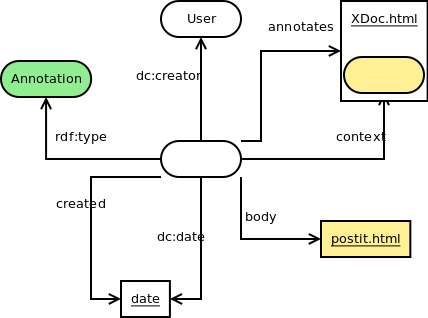
\includegraphics[width=\textwidth*4/5]{stateoftheart/rdfAnnotea.png}
		\caption{RDF model of Annotea's annotations}
		\label{overflow}
		\end{figure}
		\paragraph{}
		Annotea is open; it uses and helps to advance W3C standards when possible. For instance, we use an RDF-based annotation scheme for describing annotations as metadata and XPointer~\cite{DeRose2001} for locating the annotations in the annotated document. Similarly a bookmark scheme describes the bookmark and topic metadata.
		\paragraph{}
		Annotea is part of the Semantic Web efforts. Providing an RDF metadata-based extendible framework for rich communication about web pages while offering a simple annotation and bookmark interface. The annotation metadata can be stored locally or in one or more annotation servers and presented to the user by a client capable of understanding this metadata and capable of interacting with an annotation server over the HTTP service protocol.

	\subsection{Amaya Browser} \label{sub:Amaya Browser}
		\paragraph{}
		The first client implementation of Annotea is W3C's Amaya, a combination of a web editor and browser\footnote{\url{http://www.w3.org/Amaya/}}. Amaya is a tool used to create and update documents directly on the Web. Browsing features are seamlessly integrated with the editing and remote access features in a uniform environment. This follows the original vision of the Web as a space for collaboration and not just a one-way publishing medium.
		\paragraph{}
		Work on Amaya started at the W3C in 1996 to showcase web technologies in a fully-featured web client. The main motivation for developing Amaya was to provide a framework that is able to integrate as many W3C technologies as possible. It is used to demonstrate these technologies in action while taking advantage of their combination in a single, consistent environment.
		\paragraph{}
		Amaya started as an HTML + CSS stylesheets editor. Since that time it was extended to support XML and an increasing number of XML applications such as the XHTML family, MathML~\cite{carlisle2010}, and SVG. It allows all those vocabularies to be edited simultaneously in compound documents.
		\paragraph{}
		Amaya also includes a collaborative annotation application based on the Resource Description Framework (RDF), XLink, and XPointer as described by the Annotea standard. The Amaya browser was mainly used to showcase new features of the W3C standards and as a result the tool is specialised for the creation of hyperlinks.
		\begin{figure}[h]
			\centering
			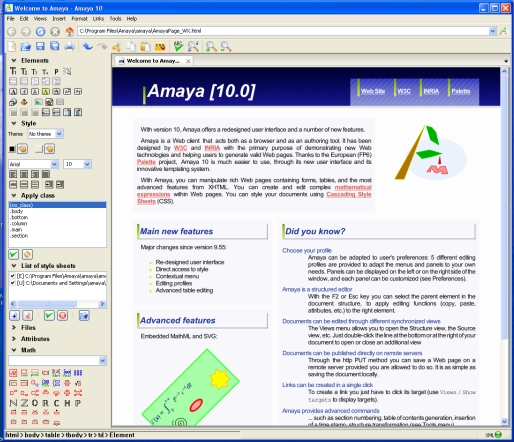
\includegraphics[width=\textwidth*4/5]{stateoftheart/amaya.jpg}
			\caption{The amaya browser}
		\end{figure}
	\subsection{Madcow} \label{sub:MadCow}
	\paragraph{}
	Madcow~\cite{bottoni2004madcow} is an acronym for \squote{Multimedia Annotation of Digital Content Over the Web} and was developed at the University of Rome: La Sapienza as a plugin for existing web browsers. The plugin uses a client-server architecture that allows users to save their created metadata to a remote server from where it can be shared with other users. The goal of the tool was to create an easy way for members of communities to share their findings and interests with each other.
	\paragraph{}
	The functionality of Madcow consist of reading, creating, saving, updating and retrieving multimedia annotations but does not allow the creation of hyperlinks between content.
	\begin{figure}[h]
		\centering
		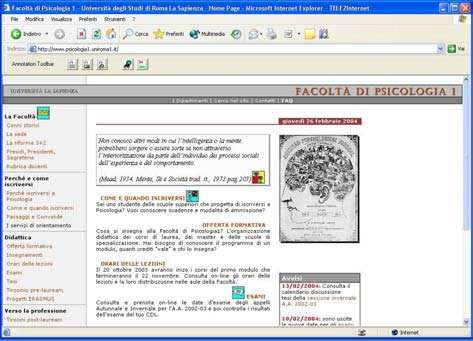
\includegraphics[width=\textwidth*4/5]{stateoftheart/madcowBrowser.png}
		\caption{The MADCOW plugin}
	\end{figure}
	\begin{figure}[h]
		\centering
		\begin{subfigure}[b]{\textwidth*2/5}
			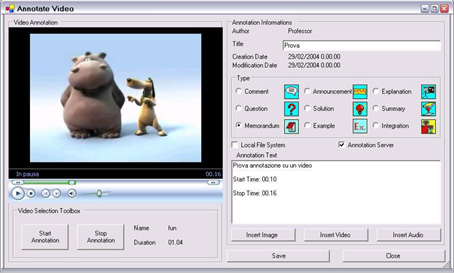
\includegraphics[width=\textwidth]{stateoftheart/madcowAnnotation1.png}
			\caption{Video annotation}
		\end{subfigure}
		\begin{subfigure}[b]{\textwidth*2/5}
			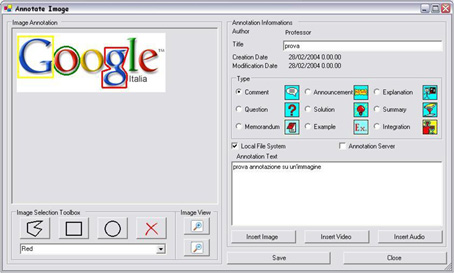
\includegraphics[width=\textwidth]{stateoftheart/madcowAnnotation2.png}
			\caption{Image annotation}
		\end{subfigure}
		\caption{Annotations in MADCOW}
	\end{figure}
	\subsection{iWeb} \label{sub:iWeb}
		\paragraph{}
		iWeb is a front end for iServer~\cite{norrie2005information}\cite{signer2008fundamental}, a collaborative metadata server that stores linking metadata for different resources. iWeb is implemented as an add-on for Firefox, enabling the user to highlight a part of the web page and create an annotation or a link to another web page. This metadata is then stored in iServer's back end. The main problem with iWeb was the fact that it was implemented as a plugin, and was therefore highly reliant on the inner workings of Firefox at that time. Web browsers tend to change their inner workings rather quickly to accommodate for changes in the web standards or to increase performance. As a result, iWeb was strongly bound to a specific version of Firefox and would not work in the future without continuous updates. Instead, we opted to start over, and make the tool as generic and independent as possible. In a way, iWeb was the predecessor of our current tool, in that it gave us a lot of valuable insights in how we could visualise the metadata on the Web.
\section{Newly Introduced Issues} \label{sec:Newly Introduced Issues}
	\paragraph{}
	One characteristic all the tools we introduced share is the fact that they were intended for a single user. At best the data is stored on a personal server, so that peers can connect to it and share their findings and even in these cases the amount of people using a single database would be fairly limited. As a result of this design decision the users can manually manage the metadata that is created. If a page becomes to cluttered the users could simply remove a couple of unneeded links, or regroup some similar ones.
	\paragraph{}
	When dealing with a truly collaborative system, where users of all backgrounds share their metadata on one large central server, this management cannot be done manual any more. These issues where previously masked because of the setting in which the tools were supposed to be used. Drastically changing the intended setting would inevitably lead to new issues that need to be addressed.
	\subsection{Visibility} \label{sub:Visibility}
	\paragraph{}
	The first major issue a multi-user system needs to deal with is the visibility of a web page. Imagine the front page of a popular newsletter website that has thousands of hits per day. A good portion of these users will have additional information to share with the community, and they will do so by creating a link to a different article. But as we can imagine, the community will soon generate such a large amount of metadata that visualising all of this data on the web page will become unreadable. When another user then views the page, it will be difficult for them to see the actual content through the seas of extra data, so the usability and readability is reduced because of the tool.
	\paragraph{}
	Most tools will visualise the origin and destination of the links within the content of the page by some form of highlighting or underlining the relevant parts of the text and since there is so much data to be visualised, it is possible that the entire document will be highlighted. A completely highlighted page is just as useful as a plain one.
	\paragraph{}
	New users will therefore arrive on a page that is completely cluttered with metadata that adds nothing to the user's experience and will actually hamper the user in the reading of the original text.
	\paragraph{}
	This means that once the amount of visitors is high enough, there is a potential danger that the system will work against itself. At that point the user would be better off not using the tool at all. Therefore a better way needs to be found for visualising the potential vast amount of metadata without overwhelming the user with too much data.
	\paragraph{}
	A second problem with trying to visualise the source and destination of the hyperlinks occurs when we have hyperlinks with overlapping sources. Two hyperlinks may be created where the source selection of the first link overlaps with the source selection of the second one. Naively visualising these two links will result in a highlighted area of text with no distinction as to where the first selection ended, or the other selection began. The same effect happens when two selections are exactly next to each other, and when one of the selections is completely within a second one. Visualising these types of scenarios directly on the page can be a challenge and may require even more metadata, such as layering, to be rendered in a readable way.
	\begin{figure}[h]
		\centering
		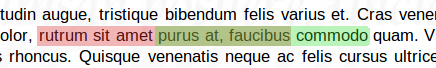
\includegraphics[width=\textwidth*4/5]{stateoftheart/Overlapping.png}
		\caption{Two overlapping selections}
		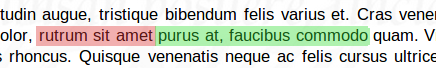
\includegraphics[width=\textwidth*4/5]{stateoftheart/Connecting.png}
		\caption{Two connecting selections}
		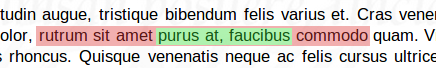
\includegraphics[width=\textwidth*4/5]{stateoftheart/Encapsulating.png}
		\caption{A selection surrounding another}
	\end{figure}
	\subsection{Scalability} \label{sub:Scalability}
		\paragraph{}
		A second major issue that was masked because the tools were intended to be used by a single user or a small group of users, is the issue of scalability. When more users are using the same shared database, the amount of metadata that the tool needs to handle increases. Searching for specific annotations or hyperlinks will become increasingly difficult. This is not only a visualisation problem but a technical problem as well. For example, the Amaya browser allows users to share a sort of bookmarks on pages, which can function as hyperlinks that are not rendered on the page. The user can then search through the bookmarks on a certain page, but when the amount of bookmarks becomes to high, more intelligent ways of searching need to be introduced to mitigate this problem.
		\paragraph{}
		The authoring of new links will become another problem that is strongly linked to the searching problem. The community would not want users to create hyperlinks that are already in the system. But if it is difficult to search whether a specific hyperlink already exists, it is difficult to detect whether the newly authored link is a duplicate or not. Therefore the tool needs to take into account that the creation of duplicates is a possibility and act accordingly.
		\paragraph{}
		This problem did not occur when the tool was only used in the simpler single user setting, because the amount of data that needs to be managed is significantly smaller than when the tools is being used by hundreds of users simultaneously.
	\subsection{Lack of Overview} \label{ssub:Lack of Overview}
		\paragraph{}
		Even in small groups of users where the metadata might not clutter the entire page, it can still cause trouble for users looking for extra information regarding a subject on the source page. For example, the users are not interested in blog posts or videos on this particular topic, instead they would like to find scientific papers that provide more information. With all the links and metadata rendered on top of the page, it is difficult for the users to find the type of links they are interested in. It might be possible that the sentences the users are interested in are highlighted, but the links point to a YouTube clip instead of the PDF file they are looking for. This problem stems again from the fact that all this metadata is simply rendered in one place and there is no real way of filtering the types of links that the users are interested in.
		\paragraph{}
		The fact that the types of links cannot be filtered, together with the fact that all the different links are rendered in the same way, results in a lack of overview of what the page actually offers in terms of extra information. But the issue does not end there: users can only look at the structure of the page, and links are rendered within this structure. Because of this limitation there is a lot of interesting information that is not easily accessible. If we want to know what different websites a particular website links to, in other words: what are the websites that are strongly correlated with the current website, it is not an easy task to find out.
		\paragraph{}
		Therefore the larger structure of the metadata is lost as we are giving preference to the structure of the page instead. As a result it is difficult to look at the big picture of the metadata, and an overview of the metadata is lacking.
	\subsection{Suboptimal Use of Data Dimensions} \label{ssub:Suboptimal Use of Data Dimensions}
		\paragraph{}
		All this metadata has a multitude of dimensions by design. For example, the domain or web page it links to, the amount of users that followed the link, the amount of links that go to the same domain from this source document, how long ago this link has been created, and much more. However, by rendering it directly on the page, most of these dimensions are not used at all. The main dimension used in this visualisation is the location of the origin of the hyperlink. When we look at a link, we know exactly where the author of this link has intended it to appear and we know that this particular piece of content provides a context for the linked document. Other than this information there is little of the extra dimensions that is used in this visualisation. Imagine the same scenario as before, where the users are only interested in scientific papers in the PDF format. One thing these tools could do is only render the metadata for links that point to PDF files or present all different types of links in a different colour. Both options have their benefits and drawbacks. In the first scenario we may find only the intended PDF links, as we requested, but this would make it so that a lot of data that is available for the user is just not shown. One particularly interesting part of the document that the user wants to read more about has no links on it. So the users might have to look for this extra information by themselves bypassing the complete goal of the tool in the first place. However it might be the case that there are some links to blog posts in this section. Even though the user prefers scientific papers, they might still be interested in other media if the first option is not available. The second option is to show all metadata on the page but use this extra data type dimension to colour code the links on the page. This results in too much data being rendered and on top of that it is rendered in all kinds of different colours, again overwhelming the users.
		\paragraph{}
		The main problem is that the visualisation uses the spatial dimension as the most important one. They render the data based on the location of the origin of the links first, and after this dimension is rendered can try to add different dimensions, such as file type. There is no way for this type of visualisation to change the priority of the used dimensions. If the user is far more interested in the type of data, and after that the location of the link in the current document, there is no way to do this.
		\paragraph{}
		Even worse is the fact that some dimensions of the metadata simply cannot be used in this way. To determine how tightly two web pages are linked together based on the amount of links between them, we can analyse the metadata using an external tool but we cannot show this information directly to the user when they are browsing the web page using these tools. This information if often requested and is available in the metadata, it just cannot be used properly because the tool gives preference to the spatial dimension before anything else.
	\subsection{Copyright} \label{sub:Copyright}
		Another feature some of the tools implement is the possibility to transclude content of hyperlinks when rendering a web page. Instead of rendering a link pointing to a paragraph, the paragraph will be rendered where the link was defined. This is a nifty feature, and it will give a more complete picture of what extra information is available through the hyperlinks.
		\paragraph{}
		Aside from the visualisation issues, a non-technical issue arises with this feature. If the tool allows transclusion of content that is not necessarily provided by someone who owns the copyright on the content and the tool then transcluded this content on another web page, it is violating the copyrights of the transcluded content.
		\paragraph{}
		Is the user not allowed to create the hyperlink between these two web pages, or is the tool not allowed to transclude the content for this particular web page? Should the tool ask the author of the web page whether he is allowed to transclude its content or not? Should there be no transclusion at all to bypass this problem from the start? These are only a handful of the issues that can arise in tools where sharing and transclusion is a core feature.
		\paragraph{}
		There is no fixed answer to these questions but this should definitely be taken into account in the design of such tools. The tool can, for instance, allow websites to specify if they would like to be transcluded or not. If no information is available for a particular website, the tool will fall back on a default of rendering a hyperlink and leave the transclusion out. The tool could also transclude the content, but make sure that the original source is mentioned in the transcluded content. These examples show that there it not a fixed solution to handle these issues. But a well defined tool can certainly help to avoid serious copyright and ownership issues.
	\subsection{Side Effects} \label{sub:Side Effects}
		\paragraph{}
		The tools work well when used on a small scale, which is their intended setting, but the benefits quickly dwindle when too many users are creating metadata in the same shared database. For a small group of users that have the same interests or look for more information in the same sources, these tools can work great. But when too many users with diverse interests are dumping data in the same database, it will most likely hinder the users more than help them. As a result, these tools are best used on a smaller scale and within closed environments.
		\paragraph{}
		If we attempt to use the tools in a real multi-user setting, all the above mentioned problems will occur sooner or later. Pages will get cluttered with metadata, resulting in unreadable websites. Looking for new information on a specific topic will be cumbersome because there is simply so much data, and no real way of filtering or searching through it. In the end people might use the tools by turning everything off until they really cannot find something they are looking for. They will then turn the system back on and go through the painstaking process of browsing through the vast amount of data to see if the information they are looking for is in the system.
		\paragraph{}
		This defeats the purpose of the tools completely and will create a cascade of negative effects on the usability of the tool. If many users find that the tool hinders their search for additional information, they will stop using the tool as intended. As a result they will most likely stop authoring additional information, which will lead to a disengagement of a big part of the community. This will result in creation of less hyperlinks. Some people will then not find the additional information they are looking for and maybe stop using the system as well. This is a self-reinforcing cycle and eventually the tool will offer no real help to most users.
		\paragraph{}
		These problems have not been addressed by existing tools simply because the tools were intended to be used by a single user. This was of course in most cases a design choice, but it masked some important issues nonetheless. We can however analyse these design choices and by doing so we identified some key issues that stem from these design choices. Taking what we have learned from other tools, we can use this information to create a tool that will address these problems and this will eventually result in a better user experience and a tool that will promote collaborative annotating and hyperlinking of web pages.

	\section{Summary} \label{sec:Summary}
	\begin{center}
		\begin{tabular}{|p{3.5cm}||c|c|c|c|c|}
			\hline 
			\rowcolor{lightgray}Technical													& HTML5 & Annotea & Amaya  & Madcow & iWeb   \\ \hline
			\hline                                                                                                \hline
			\cellcolor{lightgray}Separated Metadata File					&        & \cmark & \cmark & \cmark & \cmark \\ \hline
			\cellcolor{lightgray}Collaboration										&        & \cmark & \cmark &        &        \\ \hline
			\cellcolor{lightgray}Centralized Server								&        & \cmark & \cmark &        & \cmark \\ \hline
			\cellcolor{lightgray}Extensible												& \cmark &        &        &        &        \\ \hline
			\cellcolor{lightgray}Search Function									&        &        & \cmark &        &        \\ \hline
			\cellcolor{lightgray}Spatial Dimension Preference			& \cmark & \cmark & \cmark & \cmark & \cmark \\ \hline
			\hline                                                                                                \hline
			\rowcolor{lightgray}Visual														& HTML5 & Annotea & Amaya  & Madcow & iWeb   \\ \hline
			\hline                                                                                                \hline
			\cellcolor{lightgray}Inline Rendering									& \cmark & \cmark & \cmark & \cmark & \cmark \\ \hline
			\cellcolor{lightgray}Overlapping Selections						&        & \cmark & \cmark &        & \cmark \\ \hline
			\cellcolor{lightgray}Transclusion											& \cmark &        & \cmark &        &        \\ \hline
			\cellcolor{lightgray}Structural Overview of Metadata	&        &        &        &        &        \\ \hline
			\hline 
		\end{tabular}
	\end{center}
	\paragraph{}
	As illustrated above, all of these tools address some of the issues with the limitations discussed in Chapter \ref{cha:Limitations of Linking Techniques}. The main focus of almost all the tools is the separation of the linking metadata from the content of the document. This is not surprising and represents a major step in the right direction. The tools may also address a couple of other issues but there is no all round best solution and we will need to weigh the pros and cons to choose the appropriate tool.
	\paragraph{}
	Another interesting trait all the tools have in common, is the fact that they all render their metadata inline. This is no improvement over standard HTML and this contributes to many limitations these tools still have such as the lack of structural overview of the metadata.


%!TEX root = thesis.tex 

\chapter{An Alternative Approach} \label{cha:An Alternative Approach}
\paragraph{}
If we take what we learned from the tools we described in Chapter \ref{cha:Towards a Better Web} and try to address the identified issues these tools have, we could greatly increase a user's experience when browsing the Web and create a better network of associative links between existing content. The one big challenge we face is to make the new tool as scalable as possible while also allowing it to expand and incorporate new features when the necessary technology arises.

\section{Separation of Concerns} \label{sec:Separation Of Concerns}
	\paragraph{}
	The one positive recurring feature that most of the tools implemented was the separation of the metadata from the actual content. This movement of separating all concerns has been making its way in multiple parts of the Web as well. Most HTML elements can have a style attribute attached to them. This attribute can be inlined into the HTML like so: \code{<div style="color:red">}. This will ensure all text within this \code{div} to be rendered in red. Suppose we wanted all our \code{div}'s text to be red we could create a style element in our HTML page like so: \code{<style type="text/css"> div\{color:"red";\}</style>}. This makes the maintenance of the page a lot easier. Instead of having to change all inline styling for each \code{div} element on the page, we can just change the inline style-tag's content to achieve the same effect. However, most sites consist of multiple HTML pages and not just a single one. If we wanted to change the styling of our \code{div}s over the entire website, we would still have to manually change all the HTML files to incorporate this change. This is of course cumbersome and error prone. To remedy this problem, cascading style sheets (CSS)~\cite{Etemad2011} were invented, separating the structure and content of the page from how the page should be styled. The content and structure is described by the HTML file, while the styling is defined in the CSS file. If we now include the CSS file on each of our web pages we can simply change the styling in the CSS file and the entire website would reflect this change. Since the introduction of CSS it has become a sort of taboo for websites to style their elements within the HTML structure and it is considered bad website design if some elements have embedded styling.
	\paragraph{}
	The same evolution is happening with JavaScript files as well, moving from inline \code{<script>} tags to JS files that can be included into the page.
	\paragraph{}
	It is strange however that web standards have not yet separated the linking from the content as well. Links between different resources are still embedded into the page by means of an anchor tag. If we separate this concern from the content as well, we can change, add or remove links from a web page with the same ease as we can change its styling. This technology, however, is not yet incorporated in the current HTML standard.
	\paragraph{}
	Most of the tools discussed in Section~\ref{sec:Existing Tools} already saw the benefits of separating the content from the linking metadata and therefore save the linking metadata in a separate local file or on a remote shared database.

\section{Link Filtering} \label{sub:Link Filtering}
	\paragraph{}
	The goal of the tool is to represent the saved metadata on a web page. As discussed in the previous chapter, we need to render this metadata in such a way that the page is still readable and usable by all users. So we need to device a strategy that allows us to render a large amount of metadata on the page, without cluttering it. We will now describe a couple of approaches we can take to achieve this goal.
		\paragraph{}
		The main problem when dealing with a multi-user system of this nature, is the amount of metadata that needs to be visualised. Previous tools could ignore this problem because they were intended to be used by either a single user, or a small group of users. So a seemingly obvious way to bypass the issue of an overfull page that is not usable by the users is to filter the metadata that is rendered to a manageable amount. There are a couple of ways we can go about how filtering the total amount of links to a manageable set that can be cleanly rendered on the HTML page without overwhelming the users.

	\subsection{User Specified} \label{ssub:User specified}
		\paragraph{}
		A simple, yet effective way to weed out the excessive, unneeded links is to have the users specify what data they are interested in. The users could for example change their options in the tool to specify that they are more interested in PDF files than videos. In the same way they could ask the system to filter out any metadata that is older then 2 months because they have most likely already heard about this information by then. By filtering in this way, they ensure that the new metadata stands out in the web page so they can easily see what new information is available for the topic.
		\paragraph{}
		The amount of parameters on which users can filter their metadata can be very large. But this introduces another issue. How will the tool keep up with all the new parameters of filtering data. It is infeasible to know all the different ways to filter the metadata in advance and even if we would know these parameters, the list would be so large that it would be cumbersome for a user to configure the tool so that it will represent its needs. Off course this problem can be bypassed by having the users create their own filtering parameters too. We can take the website Twitter.com as an example for this. On Twitter a user can specify an arbitrary tag that they are interested in and if someone else on Twitter posts a message that includes this arbitrary tag the users will be notified of this. This approach has proven to be very effective for classifying metadata~\cite{macgregor2006collaborative}. A similar approach can be taken to filter the metadata for the users based on their specified tags.
		\paragraph{}
		Even though the filtering of metadata can be done more or less in the same way as Twitter does it, we need to take into account that there can be a very large set of different tags. So telling the tool how to handle each specific tag is not viable. The users could create a default fall back in case there is no rule specified for a specific tag. This would solve the problem of having to specify too many rules. But this will also result in a lot of data being hidden from the user, even though they might have been interested in this information. Imagine the users configuring the tool in such a way that the tag \squote{OrbitalPhysics} needs to be rendered and nothing else. Because these tags are so arbitrary, there might be other users tagging their metadata with the tag \squote{Orbital\_Physics}. As we can see this will cause the metadata to be hidden for the user, so they are missing information that they actually wanted to find. Determining whether two different tags are in fact synonyms is quite a problem and requires additional semantic information~\cite{marchetti2007semkey}.
		\paragraph{}
		This problem stems from the fact that the tool is used by a large community. If there was a set of rules as to how a tag needs to be formatted this particular problem would be solved. But there are many more of these scenarios that can cause the system to fail and this would result in a user either seeing data they did not intend to see, or the users might not see some information that they actually did want to see. This technique for filtering the metadata is heavily reliant on the community's tagging rules.
		\paragraph{}
		To help mitigate this problem the tool can aid the users when they are tagging their hyperlinks. The tool can auto complete while the users are typing the tag they want to add. By showing the users already some of the suggestions it is easier to select one that is fitting. The tool could query the database to find out how many hyperlinks already exist containing this particular tag. If there are two different tags that are synonymous the users can see which of the two is used more often, and then follow this trend in their own hyperlinks.
		\paragraph{}
		When a user wants to share some information with the community by means of adding metadata to a website they need to fill in as much extra metadata as possible. If the users for example neglects to specify that the hyperlink they are adding points to a PDF file, many users that wanted to see this information will not get to see the links when they visit the web page because they might filter out any link that are not pointing to a PDF file. This means that the authoring of links or metadata has a lot of overhead and becomes significantly more difficult and time consuming for the users. Ideally the tool should automatically detect as much metadata as possible to fill in for the users.
		\paragraph{}
		Since we cannot know all the different filtering criteria when creating such a tool, we cannot enforce strict rules on how the authors of a hyperlink needs to tag their metadata. Because of this, the system will be very vulnerable to spammers and malicious users who can create links to fishing websites but they might tag the link as a relevant video or something similar.
		\paragraph{}
		So there are a couple of important drawbacks of this system, but it is not without benefits. The fact that a user can specify in a very fine-grained way what they are interested in is a significant benefit. These rules are also easily changeable if the users so desire. Suppose that users are currently working on writing a thesis and they are looking for interesting papers they can use as reference. At this moment the users are not interested if the same information is also available in the form of a YouTube video. However, when the users are not looking for these papers to refer to any more and they are merely looking for the information, they might be interested in these videos too. They can then go to the configuration of the tool and change the rules that specify which type of metadata needs to be rendered.
		\paragraph{}
		The fine-grained nature of the rules combined with the ability to change the rules on demand is a very powerful way to filter out unwanted links and match the needs of the user.

	\subsection{Community Based} \label{ssub:Community Based}
		\paragraph{}
		A different yet somewhat similar way to filter the amount of links to be rendered is by relying on the community as a whole to filter the unwanted links. If a link is created and posted on a website the community will then decide whether the link is relevant to the topic of the website or not. By allowing the users of the tool to up- and down-vote these links we can attach a score to each of the created links. This score can then be used to filter irrelevant metadata from the website. The users will be able to configure their tool to set a minimum score that a link needs to have in order for it to be rendered. A user that is only looking for the most accepted or popular links will set a fairly high threshold while other users might want to see more by setting the threshold lower.
		\paragraph{}
		In the scenario where the author of the metadata has neglected to fill in some information the community could also fix this problem. If the link is relevant, but the author forgot to specify that it links to a PDF file, other users might be allowed to fill in this information in their stead. This will ensure that the links that pass the evaluation of the community will have a certain degree of hygiene with which the community is satisfied. The previously described example where a link is tagged with \squote{Orbital\_Physics} but the community expects these type of links to be tagged with \squote{OrbitalFhysics} should not happen any more. Either the link will be down-voted because it was not complaint with the community's tagging rules or the metadata will be changed by the community to make it fit their standards.
		\paragraph{}
		The beauty of this system is the fact that it is self-regulating and very stable~\cite{moore2008evaluating}. The community will decide the rules and based on these rules, links will get rated. Spammers, who will create links that span multiple paragraphs will get down-voted because of that. If several links are created on the page that all point to the same resource, the community will replace the duplicates with a single hyperlink with multiple sources instead.
		\paragraph{}
		A second benefit is that the system is democratic. The eventual result of which links are rendered and which ones are hidden will be decided by the majority of the community. A single user that has a different believe then the community cannot force his viewpoint on the community, unless a large portion of the community shares that user's vision.
		\paragraph{}
		But this is also a big weakness of the system. If the majority of the users thinks a certain links is irrelevant it does not necessarily mean this is actually the case. And someone who is looking for this less popular information will not find it. The users could possibly set their threshold significantly lower to find the information they are looking for, but they will have to go through all the rejected metadata as well and this is time consuming and defeats the purpose of filtering the bad links in the first place. This problem will become especially noticeable when multiple large groups of users have different opinions about a certain topic~\cite{sumi2011edit}.
		\paragraph{}
		Another concern we could have with this system is the fact that it punishes new content. Suppose a couple of hundred links are already on the web page and they are all considered important and interesting. That means all of these links have received a significant amount of up votes by the community. When a user finds another source of relevant information they will create a new hyperlink to that resource. But since this is a new hyperlink it has not yet received any up votes, an will therefore not be rendered for any of the users browsing the website.
		\paragraph{}
		One way to solve this problem is to decrease the amount of votes for all existing links. All existing links will be decreasing in the amount of votes at the same rate. Therefore the relative difference in votes will stay the same. New links however will have a reasonable chance of getting noticed because they will start at a fixed value of votes that does not decrease over time.
		\paragraph{}
		But this opens up the issue of spamming again. Malicious users could keep creating new links on the web page and since all other links are diminishing in votes, eventually their new links will make it to the page for other users to be seen. So the system is not perfect and spamming will still be a possibility but the effect is a lot less prominent then it was in the previous discussed alternative.

	\subsection{Machine Learning} \label{ssub:Machine Learning}
		\paragraph{}
		The problem with community based approaches like the previous two suggestions are that they, well, depend on the community and the system only works as good as the community. In certain cases this approach has proved to be very beneficial, the Reddit\footnote{\url{http;//www.reddit.com}} community or the Stack Overflow\footnote{\url{http://www.stackoverflow.com/}} karma system have ensured the websites to be filtered of malicious content quite effectively, while providing the users with quick access to the information they are looking for. However this is not always the case and for smaller communities these converging situations may not be achievable. Since we are enhancing the Web as a whole, we have to take into account the less popular parts of the Web as well. In these parts there will also be malicious users but the communities for these topics could be to small so there will be less people to correct these wrongs. The previous mentioned systems will not perform as well as for large communities.
		\paragraph{}
		Another approach may be to create a user profile based on the links a user previously followed. If the users, for example, rarely follow links that point to blog posts, the system will learn that these type of links might not need to be rendered on future pages. If we allow the users to steer the machine learning into a certain direction, by flagging certain types of links to be unwanted, the amount of metadata that is rendered can be reduced further. This method can in some way mimic the first suggestion where each user configures the tool themselves. The difference is that there is will be less overhead for the authors of links. They can still just create hyperlinks without having to fill in any additional metadata and the system will then have its own rules to determine the type of the link and detect whether or not a user might be interested in this link.
		\paragraph{}
		If the users could steer the system with suggestions of what links it should not render we can create a better filter. However it is difficult to allow links to be rendered once the system had already decided not to render them. In essence this is not a problem, the issue is that the users will not know that certain possibly interesting information is present because the algorithm blocked it from being rendered. So even if the users wanted to see this information they will never get the chance to let the system know. They could of course change their settings and re-render already blocked links, but that would defeat the purpose of the filter.
		\paragraph{}
		The same problem is also present with big search engines that try to optimize the search results based on some generated user profile. Instead of showing all results in an unbiased way, some results that are deemed uninteresting by the system will not be rendered for this particular user. In essence a user will be wrapped in a sort of information bubble, where all the information that is in the bubble will be available, but all the other information will never be shown to the user, even if they might find it interesting~\cite{pariser2011filter}.
	\subsection{On Demand} \label{ssub:On Demand}
	\paragraph{}
	As stated before the problem lies in the fact that there are too many links to be rendered on the page. This would make the web page cluttered and unusable by the reader. Any interesting metadata that is available cannot be found in the sea of data that is being created. One way to limit the amount of metadata that is being rendered is to render only the plain, unaltered page at first. The page would just be the blank vanilla page as the author has intended it to be. We could then provide the metadata on demand of the users. For example, when the users highlight a part of the text the tool sends a request to the server fetching all the metadata for the content that lies within the selection. On this selection the tool will then render the fetched metadata.
	\paragraph{}
	The benefit is that we do not clutter the page beforehand. And if the reader is not interested in getting more information about certain parts of the document, they will not be bothered with additional links. If they find a specific part of the document that they want more information about, they can easily get this on demand by selecting that part of the document.
	\paragraph{}
	It is however still possible that the selection of the users contains so many links that this small selection is already cluttered with links. The users can then narrow their selection to specify more clearly the topic they want more information about.
	\paragraph{}
	The benefit of this approach is also its downside. The fact that the users need to prompt the system for information can be cumbersome. The users might be reading a part of an article, but the community has provided hyperlinks to articles proving the falsity of this article. Unless the reader actually selects the paragraph that contains this hyperlink they will not see this additional information.
	\subsection{Conclusion} \label{ssub:Conclusion}
	\paragraph{}
		All of the discussed techniques for filtering links have benefits and drawbacks. Most of them can be used in unison reducing their drawbacks and increasing their combined benefits. For example, we can dynamically load content by making use of the users' selection but after the links are requested we can filter this data based on the users' preferences, or profile. On top of this we can even make a default filtering based on the opinion of the community to get a better selection of the relevant hyperlinks. The community could also mark some metadata as \squote{Must See} so that these links will be rendered even if the users did not select that part of the document, reducing the chance of missing vital information.
		\paragraph{}
		In conclusion all of these techniques will help reducing the amount of links that need to be rendered, but to have the most benefit it is advised to create a system that is a combination of these techniques.
\section{Link Rendering} \label{sub:Link Rendering}
	\paragraph{}
	Now that we have established some ways of reducing the amount of links that need to be rendered, we can discuss how to render the selected, relevant links. This step of the process is crucial to provide the users with a usable system that helps with finding relevant information, instead of working against the user. If the visualisation is suboptimal the information that was selected in the previous step will not be presented to the users in an optimal way and makes the tool as a whole suboptimal. Therefore we now describe a couple of different approaches that can help in the visualisation of the selected metadata.
	\subsection{In Place} \label{ssub:In Place}
	\paragraph{}
	All of the previously discussed tools render the metadata on top of the actual content. They either add small indicators that notify the users of the presence of a hyperlink, or the tool highlights the text that is associated with the link. This technique is rather easy to implement, but poses a visual issue. Even with all the work of reducing the amount of metadata to be rendered, it is still possible that a single word is the source of multiple links. Suppose that NASA is mentioned in a sentence as one of the keywords. One user might want to link to NASA's own homepage, while another user chooses to link to the Wikipedia page with more information about NASA. Both sources are relevant to the context, but it is hard to distinguish the two links if they are rendered on the same word.
	\paragraph{}
	Many tools opted for a colour code approach to distinguish between these overlapping links. This will help when two links are overlapping. The tool could for example highlight the first of link in red and the second one in green. To show the users that the overlapping part contains two links, it could highlight the top in red and the bottom in green. This of course does not scale well if more then two links are overlapping.
	\begin{figure}[h]
		\centering
		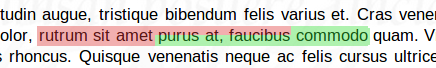
\includegraphics[width=\textwidth*4/5]{idealtool/overlapping.png}
		\caption{Overlapping links visualisation}
	\end{figure}
	\paragraph{}
	Other tools introduced layers of annotations. A link would be designated to a specific layer based on the metadata the author of the link provided. The tool will allow the users to toggle the rendering of specific layers to their liking and each of the layers will be colour coded. This does not scale well with a large amount of links either. And disabling layers will not solve the problem when two links on the same layer are overlapping.
	\begin{figure}[h]
		\centering
		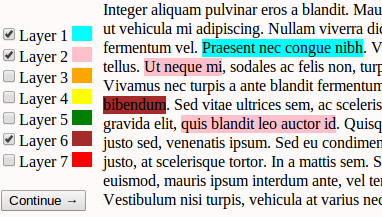
\includegraphics[width=\textwidth*4/5]{idealtool/layers.png}
		\caption{Layered visualisation}
	\end{figure}
	
	\paragraph{}
	A third option some of the tools used was to add an icon after the text on which a link exists and if multiple links are available on the same part of the text they would add additional indicators. But this would soon become an issue as well when too many links were present and therefore many icons needed to be added behind the text. A second down side was that the start of a link could not be indicated in this way.
	\begin{figure}[h]
		\centering
		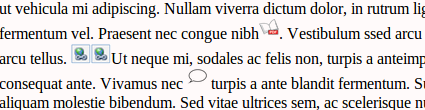
\includegraphics[width=\textwidth*4/5]{idealtool/icons.png}
		\caption{Using indicators for hyperlinks~\cite{bottoni2004madcow}}
	\end{figure}
	\paragraph{}
	Instead the tool could add icons after parts of the text that contain hyperlinks and also add an indicator of how many links are in this location. If a user clicks on the indicator a menu will open, containing the different hyperlinks. This approach will limit the amount of indicators to a minimum but does not yet address the problem of omitting the start of the link.
	\paragraph{}
	A big benefit of this approach is that the icons will replace the blue underlined text as a metaphor for the presence of a hyperlink. This is compatible with the users' way of browsing the Web, so using this technique will not drastically change how they will interact with online information.
	\paragraph{}
	Normally the destination of a hyperlink, as well as most of the other metadata, is hidden from the user. Users will just click on the blue underlined text and expect to be redirected to the associated page. Users following the link trust the author of this link that it will redirect them to a page that is meaningful to the context in which the link occurred. However in the scenario where multiple links exists on the same content a user will be prompted with a menu of links to choose from. This may not seem like a big issue, but the fact that the users need to choose between several options means that the tool must provide enough information about the different hyperlinks. The question then arises is: \dquote{How will the tool visualise the different hyperlinks in such a way that the users are presented with enough information to make an informed decision about which link to follow?}
	\subsection{Separated} \label{ssub:Separated}
	\paragraph{}
	A radically different approach of rendering all the metadata on a page is by separating the content of the page from the visualisation of the metadata. Instead of rendering the links between or on the text, the tool will create a designated area in the browser under the window in which the web page is rendered. In this area only the metadata will be rendered.
	\paragraph{}
	This approach has a couple of major benefits. The first important one is that this method overcomes the limit of the two dimensional canvas that the web page offers us. History and common web browsers have indoctrinated the idea of rendering a link on top of its context. This makes sense since an important dimension of the hyperlink's metadata is the location on which it was created. Because the simple links HTML offers us do not have a lot of dimensions there was never really a need to use different dimensions of the metadata. With the new method of creating hyperlinks many new dimensions get introduced. All of these dimensions are equally important in different scenarios. So limiting ourselves to the structure of the web page is only one way of using a single dimension to render the metadata.
	\paragraph{}
	If we decide to render the metadata in a separate window we can use all the different interesting dimensions to render the data. If we represent each web page or website as a single node in a large graph we can represent the hyperlinks as edges between these nodes. This representation lends itself exceptionally well to visualisation and using this approach we can take advantage of all the recent work in the active field of data visualisation.
	\begin{figure}[h]
		\centering
		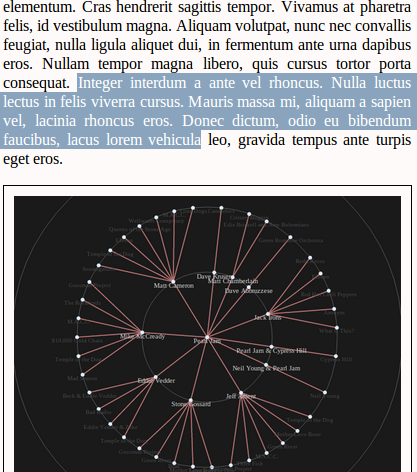
\includegraphics[width=\textwidth*4/5]{idealtool/graph.png}
		\caption[test]{Graph visualisation of metadata in selection based on JavaScript InfoVis Toolkit\footnotemark}
	\end{figure}
	\paragraph{}
	The tool will also be able to take advantage of the extra metadata that is added to the hyperlinks. Any dimension that is introduced by the metadata can be used to help with the visualisation. Nodes can be made bigger based on the popularity of the associated web page and colours can be added to represent the domain of the page. The relative positioning of the nodes can also be used to visualise another dimension of the metadata.
	\footnotetext{\url{http://philogb.github.io/jit/}}
	\paragraph{}
	Depending on the question at hand the tool can also change the visualisation from a graph to another more appropriate format. When a user wants to find a website with a strong correlation to the current page the different domains can be rendered on a radial representation as shown in figure \ref{pic:radial2}. In this image we can see 6 different domains represented by the letter A through~F. The ribbon connecting the various domains represent how strongly the two domains are linked together. As we can easily see from this one image is that the domain F is most strongly connected to the domain C since almost half of the existing links point to this domain. This information is quickly accessible for the users because of the way the metadata is presented.
			\begin{figure}[h]
				\begin{centering}
				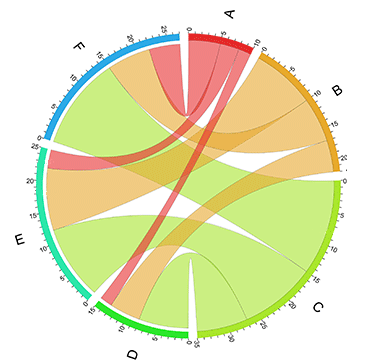
\includegraphics[width=\textwidth*4/5]{idealtool/radial2.png}
				\caption[test]{Radial Ribbon Visualisation based on d3.js\footnotemark}
				\label{pic:radial2}
				\end{centering}
			\end{figure}
	\paragraph{Zoomable}
	Because we are rendering a plain data graph we can hide a lot of complexity of the graph in large nodes. This view will provide the users with a general overview of the linking structure on the web page. Zooming in on certain parts of the graph could expand these nodes and show more detail for that particular section. For example, we could create a big node entitled \dquote{YouTube}. The size of the node will be defined by the amount of links pointing to the YouTube domain. This size will already give an overview to the users about how much information is available as video fragments. If the users are interested in a video clip about the topic they can zoom in on this one big node to show more detail. When the zoom level is sufficient the node will expand showing the different videos the page links to. This is a fairly simple example but zoom functionality can be a powerful tool to initially hide a lot of complexity for the user.
	\footnotetext{\url{http://d3js.org}}
	\paragraph{Searchable}
	The content of the graph can also easily be filtered based on some search criteria specified by the user. If the metadata is tagged as described in Section~\ref{sub:Link Filtering} the users can use these tags to filter the metadata on request. If the users are for example looking for scientific papers about orbital physics they can search the graph with these keywords as well as search for hyperlinks that are tagged as PDF. All nodes that do not fit their search criteria will be removed from the visualisation. The benefit is that the graph will still represent the structure of the metadata after the unwanted links are removed from it.
	\paragraph{}
	All of the previously mentioned filtering techniques can also be used with this visualisation. The on demand filtering described in Section \ref{ssub:On Demand} can easily be adapted to the separated view. When the users select a part of the text in the original web page the graph view will be updated in such a way that the nodes and edges represent the metadata that is found within the user's selection. Using this technique the users can easily find out if there is more information available about the context they have selected. This kind interactivity between the users' actions and the visualisation is a very powerful way of helping the users find what they are looking for.
	\paragraph{}
	Visualising the metadata in a different view that is completely separated from the structure of the web page has many benefits but there is one major drawback to this approach. The currently established metaphor of the presence of a hyperlink will be completely removed from the web page. The users can no longer look at the content of a web page and based on the blue underlined text see whether a link exists on this part of the text. And even though this may not seem like a big issue the users who have already established a way of browsing the web that works for them, will have a hard time adapting to any other way of working.
	\paragraph{}
	The users will have to keep an eye on two separated views that render two different aspects of the same content. In one frame the content is visible, while the other frame will only show the metadata. This can be confusing for new users and cause some frustration. Interaction with the metadata view could seem very detached from the web page and users will have to interact with two different views at the same time, increasing the overhead for the end user. All these effects are notable drawbacks to this approach and they should not be ignored lightly. Therefore a clear interface design needs to be established to make it easier for new users to use the tool without feeling lost because of the detachment.

\section{Link Authoring} \label{sec:Link Authoring}
\paragraph{}
Up until now we only discussed ways to visualise and filter already existing metadata. We did not yet touch the subject of how we will allow users to author their own metadata. Because we are introducing a more complex mechanism of linking resources together, it is obvious that conventional methods of creating hyperlinks will no longer apply.
\paragraph{}
In most existing tools, the users are provided with a tool bar with which they can use the authoring functionality the tool provides. Clicking a button on the tool bar will open a dedicated window for authoring. In this window the users are prompted for all additional metadata they want to provide. Typically the users are allowed to create a source selection by highlighting some text on the current page. And when the authoring window opens they are asked to input a destination URL for their new hyperlink.
\paragraph{}
Some of the tools allow the users to open new tabs, in which they can open different web pages. And when a user is authoring a hyperlink, the tool allows them to click on a tab instead of having to type the URL themselves. However, these tools do not allow the users to specify a destination selection so the authoring of the hyperlinks does not allow the users to take advantage of the full potential of the enhanced linking mechanics.
\begin{figure}[h]
	\centering
	\begin{subfigure}[b]{\textwidth*2/5}
		\centering
		$\vcenter{\hbox{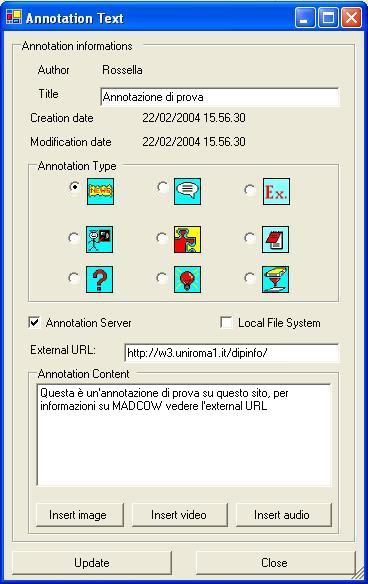
\includegraphics[width=\textwidth]{idealtool/authoring.png}}}$
	\end{subfigure}
	\begin{subfigure}[b]{\textwidth*2/5}
		\centering
		$\vcenter{\hbox{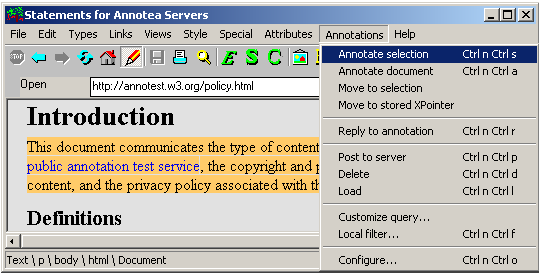
\includegraphics[width=\textwidth]{idealtool/authoring2.png}}}$
	\end{subfigure}
	\caption{Examples of authoring}
\end{figure}
\paragraph{}
We want to allow the users to author hyperlinks by navigating to the source web page and selecting the desired content. The users will then open a second tab or window in which they will navigate to the destination web page and select the content to which the link will point. Having both these selections in place the users will press a button in the tool bar that opens a window prompting them for more information. The difference is that the users are allowed to link to a specific part of a document instead of pointing to the document as a whole. This will add more flexibility and detail to the links resulting in a better experience for users looking for more information.
\paragraph{}
A third approach is to add functionality to the tool bar that allows the users to specify what role their current selection plays in the hyperlink. When the users select a part of the text they can press either one of two buttons. One will add the selection to the sources of the link, while the other button adds the selection to the destinations. This allows the users to easily construct hyperlinks with multiple sources and multiple destinations.
\paragraph{}
Each of the destinations are selections, so following a link will refer the users to the intended part of the linked document, instead of just the document as a whole. When finished the users will press a third button finishing the selection process and the tool will again prompt for more metadata, such as additional tags or comments.

%!TEX root = thesis.tex 

\chapter{The Tool} \label{cha:The Tool}
%	\section{The RSL Model} \label{sec:The RSL Model}
%	\paragraph{}
%	Hypermedia implies a lot of features. These features include semantic linking, navigational links, structural links, transclusion, annotation and context awareness. In order to realise these features, a solid foundation is needed to manage the hypermedia aspects internally. There needs to be a solid definition of how elements can be linked, how they interact and how higher levels can access the information. Such a definition can be realised through what is called a hypermedia model. Such a model is often defined without regards to implementation related aspects.
%	\paragraph{}
%	There is no shortage in hypermedia models. As early as 1994 such models have been defined, for instance the Dexter Dexter~\cite{Halasz:1994} hypermedia model. Over time this model has been extended to support time and context~\cite{Hardman:1994}, add user models~\cite{DeBra:1999} or fix implementation issues~\cite{Gron94designissues}. This is only the tip of the iceberg as many domain-specific models have been defined, some extending others and some as standalone models. We have chosen the Resource-Selector-Link (RSL) model~\cite{Signer2007}  as our basis, which is based on the OM data model~\cite{Norrie00anextended}. The RSL model is fairly recent (2007) and shortcomings and issues that were make in earlier hypermedia models have been taken into account during the development. The model provides a \emph{general platform for the development of hypermedia systems}, and is a perfect fit for the solutions that we have in mind. The resources, selectors and links can be seen as three base components for a hypermedia representation:
%
%\begin{itemize}
%\item{\underline{Resource}: A resource is a piece of data that we have in our presentation. This can be text, images or any other content type}
%\item{\underline{Selector}: When we link to a specific resources we do not always wish to refer to the entire resource. Sometimes it is necessary to refer to a specific part of the resource. For instance, a single paragraph of a long text or a small region within an image. A selector is an abstract concept that specifies a selection within a resource. Examples of implementations are for instance a regular expression for a text resource, an XPointer for an XML resource or a time interval for a video resource.}
%\item{\underline{Link}: Linking resources is the most fundamental concept of hypertext. A good model allows links to have multiple sources or targets and provides the possibility for different types of links. Resources can be linked directly, or via a selector. }
%\end{itemize}
%
%Allow us to briefly summarise some of the main features that make this model a prime candidate:
%
%\begin{itemize}
%\item{Links are first class objects}
%\item{Navigational and structural links}
%\item{User Management}
%\item{Context Awareness}
%\item{Properties}
%\item{Selectors}
%\item{Extendability}
%\end{itemize}
%
%In order to elaborate on these features we have to take a closer look at how the model defines the different components. In the following subsections we go into detail and these features will be explained along the way.
%
%\subsection{The Link Metamodel}
%
%The link metamodel is shown in \Cref{rsl_links}. The rectangles represent collections of objects of the type that is shown in the shaded part of the same rectangle. The ovals represent associations between members of collections. Note that the model is a metamodel (a model for models), and thus all the abstract concepts need to be extended in order to get a model for a specific domain (e.g.~presentations). 
%
%\begin{figure}[H]
%    \centering
%    \includegraphics[scale=0.92]{\img{rsl_links}}
%    \caption{Link metamodel (Source: Signer and Norrie~\cite{Signer2007})}
%    \label{rsl_links}
%\end{figure}
%
%In the centre of the model one can find the \code{Entity} type, which is an abstract type that is the base for the three main components in the hypermedia system: \code{Resource}, \code{Selector} and \code{Link}. \\
%
%\textbf{Resource} The \code{Resource} type represents a specific type of media. One must not forget that this is an abstract type and thus for each concrete content type that the hypermedia system needs to support (e.g.~text, images or video) one has to create an extension to this base type. This allows implementations to create plug-in systems for \emph{easy management of supported content types}. \\
%
%\textbf{Selector} A selector is an abstract concept that allows one to refer to a specific part of a resource. Again, this abstract type needs to be extended for every \code{Resource} that the hypermedia system needs to support. For instance, a type representing an XPointer expression would be a good selector for the text resource, while a temporal selector would be suited for the video resource type. The cardinality constraints imply that a selector can only refer to one resource, but a resource can be referenced by multiple selectors. \\
%
%\textbf{Link} A \code{Link} has its cardinality constraints set up in a way that allows it to have multiple sources and multiple targets. Also note that the sources and targets of a \code{Link} are of the type \code{Entity}. This implies that a link can establish relationships between resources, selectors and other links. Referring to other links can be useful for annotating other links with pieces of information. If a link points to a selector it means that it indirectly points to a part of a resource, where the selector provides the means of extracting the needed part from the resource. Because the cardinality constraints specify that a \code{Link} has at least one source and target, the model ensures that no dangling links are possible. \\
%
%On top of these core concepts the metamodel provides two useful concepts that allow additional features.\\
%
%\textbf{Properties} Properties are a set of parameters that can be associated with a specific \code{Entity}. These parameters are stored as string key-value pairs and provide a way of allowing additional flexibility for future extensions. For instance, one could allow the customisation of an entity's behaviour via these parameters in order to make it easily adaptable to other domains.\\
%
%\textbf{Context Resolver} A context resolver is an element that provides context-dependant handling of entities. Such a context resolver may grant or deny access to specific entities based on a context. Such a context could for instance be a time (a specific resource is not allowed to be accessed between specific times) or a resource type (the system may only follow links to a specific resource type, but not others). \\
%
%\subsection{The User Model}
%
%Another feature that is often lacking in other models is user management. This includes both ownership and access of information. The RSL model provides both of them via the user model as seen in \Cref{rsl_users}.
%
%\begin{figure}[H]
%    \centering
%    \includegraphics[scale=0.92]{\img{rsl_users}}
%    \caption{User model (Source: Signer and Norrie~\cite{Signer2007})}
%    \label{rsl_users}
%\end{figure}
%
%The RSL model incorporates user management at the lowest level possible. This is shown by the fact that all the user-related features are handled at the level of the \code{Entity} that we described earlier. A \code{User} is either an \code{Individual} or a \code{Group}. The concept of a \code{Group} is similar to what is offered by many operating systems. Different users have different rights, but instead of having to keep track of these rights for each user individually, groups are created as a classifier for assigning rights. For instance, in our operating system example there might be an administrator group that can do anything, a user group that is not allowed to install new software and a visitor group that is not allowed to install software or modify any settings. When a new user is created, they are simply assigned to one of the existing groups and he automatically inherits the access settings for that group. \\ 
%
%When an entity is created, it is owned by one user as defined by the cardinality of the \code{CreatedBy} relationship. The owner can then assign rights to groups or individuals, allowing sharing and collaboration. There are two relationships for assigning access rights to data: \code{AccessibleTo} and \code{InaccessibleTo}. This allows a flexible assignment of access rights as it is possible to set up complex rules. An an example of such a rule could be \dquote{\emph{Allow $group_1$, $individual_1$ and $individual_2$, but make it inaccessible to $individual_3$ (which is member of $group_1$)}}. \\
%
%Together with the \code{Context} \code{Resolvers} we described earlier it is entirely possible to set of a system of access control, securing information where needed. This user model defines the basic foundation for all features related to sharing, authoring and ownership, and is therefore well suited for use in a presentation tool. 
%
%\subsection{Layers}
%
%Earlier we mentioned how selectors can be used to access specific parts of a resource. A closer look at the link metamodel shows us that it is allowed to have multiple selectors for the same resource. This means that it is possible that two (or more) selectors resolve to overlapping content. This can be a major issue, as it is not defined how the system should handle these conflicting resolvers. Please allow us to demonstrate this issue with a simple HTML example:
%
%\begin{lstlisting}[language=XML]
%<a href="target1">
%  This is some text that links to target1, but
%  <a href="target2">
%    this text links to target2!
%  </a>
%</a>
%\end{lstlisting}
%
%One can now ask the question, if one clicks on \dquote{\emph{this text links to target2}}, will it resolve to target1 or to target2?  It is a perfect example of a situation where overlapping links cause conflicts and unless a resolve mechanism is defined, there may be unexpected behaviour. In HTML, nested links are illegal and therefore most browsers will handle this example in unexpected ways. We presented this example because even though it is illegal in HTML, it does not need to be in all hypermedia systems. The RSL model provides a solution to this problem via \code{Layers}, as illustrated in \Cref{rsl_layers}.
%
%\begin{figure}[H]
%    \centering
%    \includegraphics[scale=0.92]{\img{rsl_layers}}
%    \caption{Layers (Source: Signer and Norrie~\cite{Signer2007})}
%    \label{rsl_layers}
%\end{figure}
%
%In this model, a selector is associated with a \code{Layer} and a restriction is in place so that overlapping selectors are not allowed to be associated with the same layer. The vertical bars in the \code{|HasLayers|} relationship indicate that this is a ordered association, meaning that the layers have a particular order. If a problem with overlapping selectors arises, the selector associated with the top layer is selected and used, resolving all issues. \\
%
%One could say that this approach is restrictive, because what if one does not want the selector associated with the top layer to be selected, but instead wishes to use another one in some contexts. That is where the \code{Active Layers} collection comes into play. Layers can be marked as active or inactive via their membership in the \code{Active Layers} collection. Inactive layers (not associated with the \code{Active Layers} collection) are simply ignored allowing selectors in lower layers to be selected. On top of that, the layers can be reordered dynamically enabling applications to change the order (and thus selector) depending on the context.
%
%\subsection{Structural Links}
%
%Earlier we have described the link metamodel, but there all links have the same type, namely \code{Link}. The RSL model extends this type further by proving two subtypes of links, \code{Navigational Link} and \code{Structural Link}. \\
%
%\textbf{Structural Links} are links that tie information together to form structures. For instance, a book has structure, it has chapters, sections and paragraphs. Structural links can for instance be used to represent such a book-like structure, by defining structural relationships over the different resources. \\
%
%\textbf{Navigation Links} are links that drive the navigation in one way or another. An example of that are the HTML hyperlinks everyone knows. These are visualised in a way that the user can interact with, in order to guide the navigation. \\
%
%The definition of these two link subtypes can be seen in \Cref{rsl_structures}. \\
%
%\begin{figure}[H]
%    \centering
%    \includegraphics[scale=0.92]{\img{rsl_structures}}
%    \caption{Layers (Source: Signer and Norrie~\cite{Signer2007})}
%    \label{rsl_structures}
%\end{figure}
%
%A \code{Structure} is composed of one or more \code{Structural Links} and defines a structure over information. A structural link is simply a subtype of \code{Link} that refers to one or more \code{Entities} via the \code{|HasChild|} relationship. The \code{|HasChild|} relationship is again an ordered relationship. This is needed because a structure implies that there is a certain order and grouping. In the case of a book-like structure, as the one mentioned earlier, we have chapters that need to be ordered in a fixed way that makes sense for the content. It is not only possible to define structures over data, but it is also allowed to define structures over structures. This allows one to build more complex structures that are composed of smaller substructures. For instance, a book has chapters, a chapter has sections and a section has paragraphs. This is a case of nested structures that could not have been achieved with just structures over data, as this would just result is a flat sequence of ordered elements. Note that this concept is very beneficial for transclusion, as it would allow references to be made to structures or substructures instead of just resources. For instance, one could transclude a single paragraph or section from a book into another document. Finally, it is noteworthy to mention that it is also possible to define structures over links. For instance, navigational links can be structured to form navigational paths that will guide a viewer through the information.\\
%
%\subsection{Implementation of the RSL Model}
%
%The RSL model has been implemented in the form of a hypermedia server called \mbox{iServer}~\cite{signerphd}. iServer provides a Java API which allows easy access for applications. In order to support the needed media types a lot of resource plug-ins have been defined with their corresponding selectors. \Cref{iserver_plugins} shows some of the media types that have been implemented, together with the selector that is used for that resource. \\
%
%\begin{table}[h]
%\centering
%\begin{tabular}{| l | l | l |}
%\hline
%Medium & Resource & Selector \\ \hline
%paper & document page & shape \\
%web page & XHTML document & XPointer \\
%movie & mpeg file, avi file etc. & time span  \\
%movie & mpeg file, avi file etc. & shape \\
%sound & mp3 file, wav file etc. & time span \\
%image & gif gile, jpeg file etc. & shape  \\
%database & database workspace & query  \\
%physical object & RFID space & RFID tag  \\ \hline
%\end{tabular} 
%\caption{iServer plug-ins}
%\label{iserver_plugins}
%\end{table}
%
%\subsection{Conclusions on the RSL Model}
%
%In the previous sections, we have detailed the RSL model and discussed the major components in detail. The combined model can be seen in \Cref{rsl_complete}.
%
%\begin{figure}[H]
%    \centering
%    \includegraphics[width=\textwidth]{\img{rsl_complete}}
%    \caption{Complete RSL model (Source: Signer and Norrie~\cite{signeripaper})}
%    \label{rsl_complete}
%\end{figure}
%
%Overall, we believe that a hypermedia model such as the RSL model is a solid solution for many of the problems associated with slideware. In this section we have taken a closer look at the RSL model and have discussed a lot of concepts that will provide the necessary features that are needed to tackle some major issues present in modern slideware tools. To end this section on the RSL model, we quickly recapitulate the offered concepts and their implications on our presentation tool.
%
%\begin{itemize}
%\item{The RSL model allows us to step away from hierarchical representations and instead organise information in a graph-like structure. Instead of storing information in structured documents, a hypermedia system can be seen as a respository for resources. A presentation would merely be a navigational path through the resources in one's personal repository. All hypermedia functions can be achieved with the RSL model: transclusion, annotation, navigational links, structural links and more. This opens a lot of doors regarding how information is stored, visualised and managed for presentations.}
%\item{Hypermedia does not need to be a chaotic graph of linked resources. The structure functionality allows us to define structure where needed. }
%\item{The RSL model provides user management at the core level. This makes features possible such as collaboration, sharing and security. }
%\item{The RSL model is easily extendable with new media types and selectors to suit the needs of modern presentations. }
%\item{The RSL model was designed with real-life applications in mind, and enough functionality is built in to suit all possible needs. For example, context-awereness is built in at the core level, and special care has been taken to make the model customisable and extendable, ensuring that the model is usefull in the long term. }
%\end{itemize}

%------------------------------------------------------------
%------------------------------------------------------------
%------------------------------------------------------------
	
	\paragraph{}
	In Chapter \ref{cha:An Alternative Approach} we discussed different approaches for each aspect of the tool. Each with its own benefits and drawbacks. In this chapter we will define a concrete design for our tool based on our findings from the previous chapter. We decide on the implementation-specific details such as tools and technologies we will use. In Chapter \ref{cha:Implementation} this design is then used to build a working prototype for our envisioned tool.

	\section{Tagging Metadata} \label{sub:Tagging Metadata}
	\paragraph{}
	Based on our literature study and our personal findings we have decided that allowing the user to tag his metadata with arbitrary strings allows for the most flexibility. Users can use these tags to provide more information about the content or type of the hyperlink.
	\paragraph{}
	The reason we decided on allowing arbitrary tags instead of a fixed amount of predefined keywords is that this approach is a lot more extendible. At the time of development we can not foresee all possible ways of filtering the metadata, or preferences of the users. Therefore allowing the users to choose any string will allow them to come up with their own techniques for data classification.
	\paragraph{}
	To mitigate the issues with this technique, described in Chapter \ref{cha:An Alternative Approach}, we will provide the user with more information about the tags he is adding. When the user types a string he wants to use as a tag, the tool needs to provide a list of similar tags, that already exist in the system. This will help prevent multiple similar tags to exist, which will in turn help the users to search more effectively;
	\paragraph{}
	The tool will also keep track of the amount of hyperlinks that carries a certain tag, and this amount will be displayed next to the tag during authoring of the link. This way we can sort the list of similar tags based on their popularity, which will help the author of a hyperlink decide which tag he will use.
	\section{Selection} \label{sub:User Selection}
	\paragraph{}
	We did not find a clear advantage to either of the three options for adding a selection to the sources or destinations of a hyperlink but we agreed that allowing the user to point to a specific part of the document, instead of to the document as a whole, is an important requirement. Therefore we opted to implement all three designs for adding a selection to a hyperlink. Based on the users need he can then choose what technique he will use.
	\begin{itemize}
		\item \textit{Automatic:} The user opens two frames, and creates a selection in each of them. The tool will the decide which of the two frames will take up the role of the source, and which frame will function as the destination. This choice will be the from left to right, as we would intuitively expect.
		\item \textit{Manual:} If more than two frames are open, the user will be able to select, for each frame, what role the frame will play in the hyperlink. The selection in each frame will then correspond with the given role. This will be easier to create hyperlinks with multiple sources or destination.
		\item \textit{Manual with multiple selections:} The user can also create a selection in a frame, and for this selection decide what role it plays by clicking a button in the tool bar. The selection will then disappear leaving room for a second selection. This allows the user to easily create links where the source and destinations point to the same document. Or when multiple sources of the hyperlink decide on a single page.
	\end{itemize}
	\paragraph{}
	So based on the current scenario the user will have a couple options to finish his task. Each with different advantages and drawbacks. The more powerful techniques will require more effort from the user, while the more easy approach will only allow the user to create the most basic hyperlinks.
	
	\section{Visualisation} \label{sec:Visualisation}
	\paragraph{}
	When experimenting with different approaches for visualising the metadata we ended up choosing the approach that separates the metadata from the content because this technique is the most extensible and provides the most functionality for the end user.
	\paragraph{}
	As a proof of concept we will already implement a couple of visualisations with which the users can interact to find useful additional information.
	\begin{itemize}
		\item \textit{Radial Graph} Each node in the graph will represent a web page or resource that is the destination of at least one hyperlink of the page. The size of the nodes will indicate the popularity of the web page and is calculated by the amount of users that follow a link to that web page from the active page. It is therefore possible that the same resource will have a different popularity when visiting a different page. All nodes that represent pages from the same domain will be grouped together in clusters around the centre node, representing the active web page, and the size of the clusters will already give an indication of how tightly the two domains are correlated to each other. As a third dimension we will colour code the nodes based on the type of resource that is linked. All PDF-files will be shown in the same colour as well as the video resources and web pages. This will help the users to easily find the type of resource they are looking for.
		\item \textit{Ribbons} Each of the partitions of the outer circle will represent the domains of the outgoing hyperlinks. The ribbons between the partitions will show the amount of hyperlinks going between them and the size of the ribbon is determined by the amount of hyperlinks. This will show how tightly two domains are linked together and shows which other websites might be interesting to read to find more on the topic.
		\item \textit{Location} Each of the nodes will represent a web page or resource that is linked to. The location of the website will be rendered on the map. This can be interesting to find websites of a specific country. This visualisation is more a proof of the extensibility of the tool.
	\end{itemize}
	\paragraph{}
	To minimize the previously described issue that users might have with the separation between content and metadata we opted to still render a minimum amount of metadata inline as well. When users have two frames open next to each other and there are hyperlinks going from the content of the first frame pointing to the content in the second frame, the tool will render these hyperlinks on the content. This will bridge the gap between between content and metadata because the users can easily see where hyperlinks exists on the page as well as where the destination points to.
	\section{Interaction} \label{sec:Interaction}
	\paragraph{}
	The interaction is strongly connected to the way the metadata is visualised each of the different visualisations offer different functionality and therefore need different ways to interact with them. The most obvious of the visualisations is the radial graph representation. We expect, therefore, that this visualisation will be used for the majority of the tasks and needs an intuitive way to interact with it.
	\paragraph{Pan and Zoom}
	Browsing through the graph can be done using the pan and zoom features. Clicking and dragging on the background will move the graph accordingly while scrolling up or down on the mouse will will zoom the graph in and out. When the visualisation is zoomed out too far the clusters of resources will be grouped to a single larger node representing all of the smaller nodes and zooming back in on one of the nodes will expand it to the original cluster of nodes. This helps to keep a macro overview over the structure of links and when the users need more specific information they will zoom in to find a specific page.
	\paragraph{Search}
	When the users are looking for metadata that is tagged with a specific keyword they will enter this information in the search field. This will filter the graph with this information making it easier for the users to find what they are looking for. There will also be a couple of build in filters available for the user to use, such as filtering by popularity or how recently the hyperlink was created. These additional filters can easily be extended if the need arises.
	\paragraph{Clicking}
	Once the users have found the node that represents the web page they want to visit they will click on the node. Left clicking on the node will open the associated web page in the current frame while clicking with the middle mouse button opens a new frame with the requested web page.
	\paragraph{}
	In the ribbon visualisation panning and zooming the interface does not make a lot of sense and clicking the partitions or searching for tags is not really relevant in this representation either so these ways of interacting will be disabled. If the users want more information about one of the ribbons they can hover their mouse pointer over one of them. This will highlight the related partitions on the circle and present the users with some statistics in the form of a tool tip on the selected ribbon.
	\section{Tools} \label{sub:Tools}
	\paragraph{}
	With these requirements in mind for the visualisation we take a look at the possible candidate tools that will help us with achieving our goal. For each candidate we will mark the negative aspects (Marked with \dquote{\xmark}) as well as the positive aspects (Marked with \dquote{\cmark})\\

	\textbf{Flash / Flex}
	\begin{itemize}
		\item[\xmark]{We have no experience with Flash and related technologies } 
		\item[\xmark]{Requires a platform dependent runtime library to be installed}
		\item[\xmark]{Flash is not based on open standards}
		\item[\xmark]{Flash is slowly fading out in desktop environments since the introduction of HTML5}
		\item[\cmark]{Lots of built-in GUI elements}
		\item[\cmark]{Cross-platform (except for Apple's iOS)}
		\item[\cmark]{High level support for animation}
	\end{itemize}
	\textbf {Plain JS and HTML5}
	\begin{itemize}
		\item{\xmark} This will take a lot of time and effort without really contributing to the thesis
		\item{\xmark} While fluent graphics are well underlay, pure JavaScript is not sufficient (yet) for complex visualisation
		\item{\cmark} We can build everything from the ground up optimizing the visualisation to our requirements
	\end{itemize}
	\textbf {Sigma.js}
	\begin{itemize}
		\item{\xmark} Specialised for graph visualisations and no other form of data
		\item{\xmark} Operates in a HTML canvas element but this makes us lose most of the benefits HTML offers
		\item{\cmark} Very powerful graph rendering library
		\item{\cmark} Quite lightweight so it scales fairly well for large graphs
		\item{\cmark} Especially designed for interactivity
	\end{itemize}
	\textbf {infovis}
	\begin{itemize}
		\item{\xmark} Not as lightweight as other alternatives
		\item{\cmark} Very powerful data visualisation library
		\item{\cmark} Specially designed for interactivity
		\item{\cmark} High level support for animation
	\end{itemize}
	\textbf {d3}
	\begin{itemize}
		\item{\xmark} Because the library uses DOM manipulations animations can be slower then other alternatives
		\item{\cmark} Very powerful data visualisation library
		\item{\cmark} Specially designed for interactivity
		\item{\cmark} Quite lightweight so it scales fairly well for large graphs
		\item{\cmark} High level support for animation
		\item{\cmark} Data driven
		\item{\cmark} Flexible in usage and applications
	\end{itemize}

	\paragraph{}
	Ultimately InfoVis, Sigma.js and d3.js are almost equal candidates but in the end we have chosen to use d3.js for the following reasons.
	\begin{itemize}
		\item Instead of providing a packet deal solution the way Sigma.js does for graph visualistion, d3.js provides an extensive API that provides building blocks to build any visualisation the developers can come up with. The range of possibilities is only limited by the imagination of the creators of visualisation. This is of course what we are looking for when we want to present the metadata to the users in different ways.	
		\item The library allows us to define different visualisations for a single dataset and this matches exactly what we are trying to accomplish. When the users are interested in answering a specific question about the metadata they can simple choose the appropriate visualisation. D3.js' data driven nature matches the needs of the tool perfectly.
		\item d3.js is not limited to a canvas like some of the other alternative and this allows us to manipulate any part of the DOM structure of the web pages as well. This is especially beneficial because we can combine different already well established web technologies with the data visualisation as well which provides even more extensibility for the future.
		\item Finally, d3.js' API is better documented then the alternatives. And since there is a very active community that uses d3.js there are a lot of examples and experiments that are readily accessible. This will give us a head start when we are implementing our specific visualisations.
	\end{itemize}

%!TEX root = thesis.tex 

\chapter{Implementation} \label{cha:Implementation}
	\paragraph{}
	In Chapter \ref{cha:An Alternative Approach} we defined a set of requirements for our ideal tool and in Chapter \ref{cha:The Tool} we continued to describe our approach to achieve those requirements. Now that we have established our approach we can take this high level design and create a working implementation for it. In this chapter we will explain how we implemented our design and go into more detail on the important choices we had to make. Next, we will go over each major component of our tool and describe the technical aspect in more detail. Finally we will list some important issues we ran into when designing and developing our tool and we will suggest some work around or solutions.
	\section{Data Management} \label{sec:Data Management}
	\paragraph{}
	In our local JavaScript database we will create a simplified version of the RSL~\cite{SignerDOC}~\cite{Signer2007} model. Our tool is designed to work on web resources so there is no need to support additional media types. We will make sure that the local database is compatible with the actual RSL model to make extending the tool to an external RSL server fast and painless. In this section we will give a short description of the local database.
	\paragraph{}
	The \code{Resource} table contains the web resources that can be linked to and is identified by a resource descriptor, in our case this is the URL of the web resource, which will be the same in an RSL database. A \code{Selector} table is linked to the resources and defines the part of the document that will be selected as the source or destination of a hyperlink, in our case the selectors will be defined by an Xpointer on the web page. The \code{Selector} table also keeps a reference to the associated resource. Finally we have the hyperlinks themselves which are saved in two separate tables one table contains the sources of the hyperlinks, while the second table contains the destinations. This will allow us to easily save hyperlinks with multiple destinations and multiple sources. Both of the tables will have a field with a number that identifies the hyperlink. That way we can actually combine the information from both tables. We will also keep a \code{Hyperlink} table that joins the both the destinations and the sources. In this table we can also add more information such as the creator of the hyperlink or the date on which it was created.
	\paragraph{}
	These five tables will provide a means to save all hyperlinks in our simplified version of the an RSL database. In Chapter \ref{cha:An Alternative Approach} we discussed the need for tags on our metadata as well. To save this additional information we need an extra table named \code{Tag}. Tags will be saved in a separate table, and when a selector is created with a tag this information is saved in a join table \code{Selector\_Tag}. When a new tag is used that did not exist yet, a new entry is added in the Tag table. The amount of times a tag is used is then easily calculated from this table and this gives us an easy way to provide the users with a list of already existing tag names.
	\paragraph{}
	With this database in place we are able to store all the information we need to create the hyperlinks between different resources. This database is also compatible with the RSL model so migrating the data to a remote database poses no real difficulty.
	\begin{figure}[h]
		\centering
		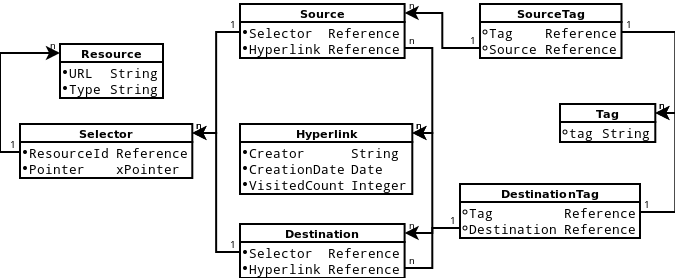
\includegraphics[width=\textwidth]{implementation/database.png}
		\caption{Model Of Local JS Database}
	\end{figure}
	\paragraph{}
	The implementation of this database will be done using HTML5 local storagei, this local storage is a simplified version of SQLite~\cite{owens2006definitive} implemented in JavaScript.
	\paragraph{}
	To make our life easier in the future we start with creating a \code{Database} prototype for which we can define methods to handle the communication with the low level database.
	\begin{lstlisting}[language=JavaScript]
var Database = function(){
	var myDb = false;
}
	\end{lstlisting}
	We can now define our methods on this database prototype
	\begin{lstlisting}[language=JavaScript]
Database.prototype.SomeMethod = function() {
	...
}
	\end{lstlisting}
	\paragraph{Set-up}
	The first thing we need to do is create a client side database if the database not yet exists so we define the \code{initDB} method as follows
	\begin{lstlisting}[language=JavaScript]
Database.prototype.initDB = function() {
	try {
		if (!window.openDatabase) {
			alert('Databases are not supported in this browser.');
		} else {
			var shortName = 'DEMODB';
			var version = '1.0';
			var displayName = 'DEMO Database';
			var maxSize = 1000000; // in bytes
			this.myDb = openDatabase(shortName, version, displayName, maxSize); //creation of DB
			this.createTables();
		}
	} catch(e) {

		if (e == 2) {
			// Version number mismatch.
			console.log("Invalid database version.");
		} else {
			console.log("Unknown error "+e+".");
		}
		return;
	}
}
	\end{lstlisting}
	\paragraph{}
	Running \code{Database.initDB()} creates the database and already makes a call to \code{Database.createTables()} which is defined as follows
	\begin{lstlisting}[language=JavaScript]
Database.prototype.createTables = function(){
	this.myDb.transaction(
		function (transaction) {
			var queries = [
				  'CREATE TABLE IF NOT EXISTS tableName('
						 ... //table column definitions
				+ ');']
			for (var i = 0; i < queries.length; i++) {
				transaction.executeSql( queries[i], [], this.nullDataHandler, this.errorHandler);
			};
		}
	);
}
	\end{lstlisting}
	\paragraph{}
	As we can see, the database framework makes use of transactions that are called on the database using a callback function. The database framework uses these transaction callbacks because the database is queried asynchronously. This means that when we launch a query in our code we will not get a response in the same way a desktop application would from a MySQL\cite{dubois2008mysql} database, instead the executing of the program continues independents of when the query will produce a result but when the query finishes the callback is then called on the result. 
	\paragraph{}
	In the previous snippet the \code{nullDataHandler} and \code{errorHandler} are both callback functions and are called when respectively the query succeeds, or fails. Since we do not need to execute any code once the tables are created we provide the \code{nullDataHandler} which just returns.
	\begin{lstlisting}[language=JavaScript]
Database.prototype.nullDataHandler = function (transaction, results) {
	console.log(results);
}
Database.prototype.errorHandler = function (transaction, error) {
	alert("Error processing SQL: "+error);
	return true;
}
	\end{lstlisting}

	\paragraph{}
	To send a query to the database we use the \code{executeSql} function as shown earlier. The following code allows us to select all the selectors that are defined on a single resource
	\begin{lstlisting}[language=JavaScript]
Database.prototype.getSelectors = function(resourceIdentifier, callback){
	var db = this;
	this.Db.transaction(
		function (transaction){
			transaction.executeSql("SELECT * FROM selector where resourceId = ? ;", [resourceIdentifier], db.resultHandler(callback));
		}
	)
}
	\end{lstlisting}
	\paragraph{}
	When we call this function we can provide a callback function which is then executed on the resulting dataset. 
	To send a query to the database we use the \code{executeSql} function which takes a query string as input and sends the query to the selected transaction.
	\begin{lstlisting}[language=JavaScript]	
DEMODB.transaction(
  function (transaction) {
    transaction.executeSql("SELECT * FROM page_settings;", [], dataSelectHandler, errorHandler);
  }
);
	\end{lstlisting}
	
	\section{Visualisation} \label{sec:Visualisation}
	\paragraph{}
	Based on our findings and experiments from Chapter \ref{cha:The Tool} we opted to go for the d3.js framework to visualise the metadata in a separate view. We chose this approach over the others because of its flexibility and data driven nature.
	\paragraph{}
	d3.js fits our needs perfectly because it maps a set of metadata to elements on a web page. We can use this to represent each piece of data as an SVG element in a separate view on the web page. When the data then changes the visualisation will mimic these changes as well. Searching and filtering the data and visualising the result will be easy since the framework already takes care of most of the work. The only thing we need to provide is a description of how we want to map a data point on the visualisation and some animation definitions for entering and exiting the representation.
	\paragraph{}
	This is an elegant and powerful way to represent the data that is stored in the database but, more importantly, it does not restrict the visualisation options in any way. Representing the data on a world map is just as easy as creating a cloud of nodes with different sizes.
	\paragraph{}
	This flexibility is so important for us because we want to allow the users to utilise all the different dimensions of the metadata as optimal as possible and we can only achieve this if we are able to generate many different views for the same data.
	\paragraph{Forced Directed}
	The data driven nature of the framework allows us to first collect all the needed data in an array, on which we then apply a predefined visualisation. For the forced directed layout we need two data array. One containing the nodes of the graph, which are the resources that the current page is linking. The second array will contain all the actual hyperlinks between all the selected resources.
	\begin{lstlisting}[language=JavaScript]
var resource = getResourceIdentifier();
var nodes=DB.getResourcesLinkedTo(resource);
var edges=DB.getResourceLink(resource);
var color = d3.scale.category20();

	\end{lstlisting}
	\paragraph{}
	Once we have collected all the required data, we need to build the layout with the correct parameters. Proving a link distance and a negative charge to the nodes will allow the layout to calculate the final positions of the nodes. We bind the nodes and links of the visualisation to the nodes and edges we have previously retrieved from the database.
	\begin{lstlisting}[language=JavaScript]
//initialize the d3 force layout
var force = d3.layout.force()
	.nodes(nodes)
	.links(edges)
	.charge(-120)
	.linkDistance(30)
	.size([width, height]);

//create the svg canvas in the visualisation div
var svg = d3.select("visualisation").append("svg")
	.attr("width", width)
	.attr("height", height);

	\end{lstlisting}
	\paragraph{}
	Now that we have mapped the data to the visualisation elements we need to do the opposite as well. The following code snippet show how we can map the selected visualisation elements in the \code{svg} container to the data arrays we have previously saved. On this mapping we can then create enter, exit and update procedures. The enter procedure described for the edges will execute when there is a mismatch between the visualised elements and the data elements stored in the \code{edges} array. When an element is present in the data array but not in the visualisation the layout will  create a new \code{line} element and provides the correct attributes to it, effectively rendering it in on the page and restoring the synchronisation between the two representations. The exit procedure will execute when the missmatch between the two array suggest that there is an element in the visualisation that is no longer present in the data array and when this happens the layout will remove the element from the \code{svg} element.
	\begin{lstlisting}[language=JavaScript]
//map edges array on the data elements of the visualisation
var link = svg.selectAll(".link")
    .data(edges)
  //enter behavior for new edges
  .enter().append("line")
    .attr("class", "link")
    .style("stroke-width", function(d) { return Math.sqrt(d.value); })
  .exit().remove();

//map nodes array on the data elements of the visualisation
var node = svg.selectAll(".node")
    .data(nodes)
  //enter behavior for new nodes
  .enter().append("circle")
    .attr("class", "node")
    .attr("r", 5)
    .style("fill", function(d) { return color(d.group); })
    .call(force.drag);

	\end{lstlisting}
	\paragraph{}
	Finally we need to specify how the visualisation will change on each moment in time. In this code snippet we specify that at each tick the coordinates of the endpoints of the edges should correspond with the position of their respective nodes in the graph. It also specifies that the location of the node elements on the visualisation should match the location that is provided in the data array. Since the force layout changes the information in the data array we need to manually maintain this synchronisation.
	\begin{lstlisting}[language=JavaScript]
//tick behavior
force.on("tick", function() {
  link.attr("x1", function(d) { return d.source.x; })
    .attr("y1", function(d) { return d.source.y; })
    .attr("x2", function(d) { return d.target.x; })
    .attr("y2", function(d) { return d.target.y; });

  node.attr("cx", function(d) { return d.x; })
    .attr("cy", function(d) { return d.y; });
});
	\end{lstlisting}
	\paragraph{}
	The only thing that is left to do now is kick it all into action by starting the layout.
	\begin{lstlisting}[language=JavaScript]
force.start();
	\end{lstlisting}
	\paragraph{}
	The resulting visualisation will show a graph representation of the interlinked resources that will dynamically update when the data array is manipulated as shown in figure~\ref{fig:forceDirected}
	\begin{figure}[h]
		\centering
		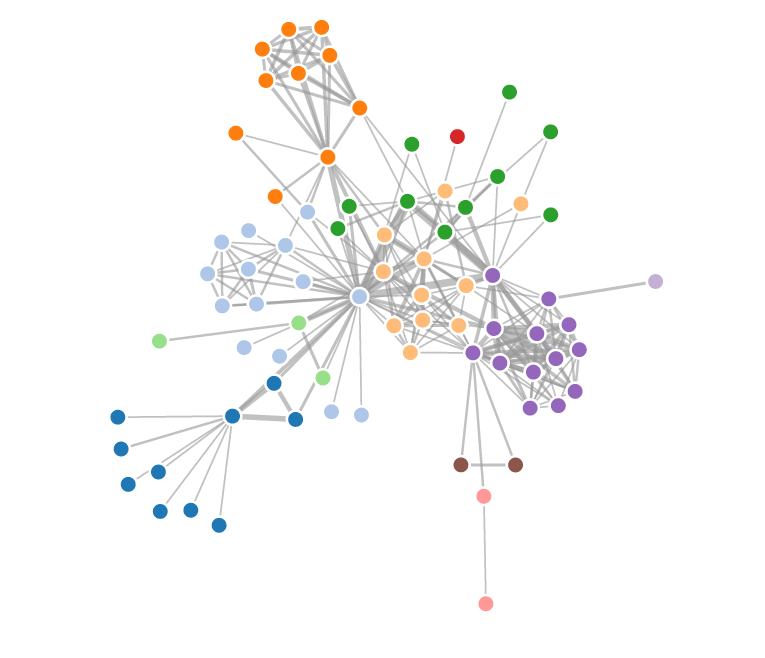
\includegraphics[width=\textwidth*4/5]{implementation/forceDirected.png}
		\caption{Force directed graph of web resources with their hyperlinks}
		\label{fig:forceDirected}
	\end{figure}
	\paragraph{}
	Many other visualisations can be created with this bidirectional mapping between visualisation elements and data elements and as we can see, the framework allows us to exploit very different dimensions of the same dataset in many completely different ways. This will help the users to find the correct information, or answer questions about the general structure of the metadata.
	
	\section{Interaction} \label{sec:Interaction}
	\paragraph{}
	Now that we know how to save and retrieve the data and visualise this data in many different ways, we need a way to allow the user to create the metadata and once the data is rendered the users need to be able to manipulate this data.
	\paragraph{}
	The users are able to create a selection on a web page using their cursor and save this selection as a \code{selector} to use as the source or destination of a hyperlink. To aid us with the management of user created selections we make use of \emph{Rangy}\footnote{\url{http://code.google.com/p/rangy/}}, a JavaScript library that supports many abstractions for creating, serialising and restoring user created selections.
	\paragraph{}
	First we want to allow the users to select a part of the web page which we can capture with the \code{getSelection} method \code{Rangy} provides us. The resulting object is an XPointer representation of the users' selection which we need to serialise to save it to the database. When we want to render the selection back on the web page again we need to de-serialise the saved selection and use the resulting selection object to add indicators on the web page on which we can apply CSS styles.\\
	\begin{lstlisting}[language=JavaScript]
		//saving
		var sel = rangy.getSelection();
		var serializedSel = rangy.serializeSelection(sel);

		//restoring
		var cssApplier = rangy.createCssClassApplier("Selection"});
		var sel = rangy.deserialiseSelection(serializedSel);
		cssAppier.applyToRange(sel);
	\end{lstlisting}
	\paragraph{}
	Now that we can save and serialise the users' selection we only need to allow the users to select a particular piece of text and choose whether the selected text is the source or destination of the hyperlink that is being created.

	\section{Concerns} \label{sec:Concerns}
		\paragraph{}
		In this section we will discuss the setbacks and issues we have encountered while developing the tool.
		\paragraph{Dynamic Content}
		More and more websites are becoming interactive where a single web page will generate different content based on some value in the users' cookies or some server-side parameters. If users create a selector on a resource which is defined by its URL this relation is saved in the database. When the users then visit the same web page the database will be queried for all relevant selectors and since we had saved one before we will find at least one. This selector is defined by the XPointer that is saved in the database but when the tool tries to render this XPointer on the generated content there is no guarantee that the XPointer is still valid. This problem is even more noticeable on so-called \dquote{Single Page Websites} where all the content is requested with AJAX(CITE) calls and is then dynamically loaded on the web page.
		\paragraph{Same Origin Policy}
		The Same Origin policy is an important security concept for a number of client side programming languages, most notably JavaScript. The policy states that only scripts originating from the same host as the web page itself, are allowed to be executed on that page. Being the same host is then defined in terms of the scheme, host name and port number of the web page. The issue with our tool is that our JavaScript will be requested from a different domain than the web pages. The tool request the content of a web page from its actual server to get the latest version of the content and with this content loaded in a frame we use our JavaScript to manipulate the DOM structure of the document. This will be blocked by the same origin policy which does not allow our scripts to run on the document structure of another web page.
		\paragraph{X-Frame-Options}
		The X-Frame-Option header that can be set by the server is a mechanism developed by Microsoft in January 2009. This header option is intended to protect users against click jacking attacks. Click jacking, or User Interface Redressing is a malicious technique of tricking a user to click on something different than what the user intended to click on. This is accomplished by loading the content of a legitimate website in a frame, and then rendering a transparent layer on top of the other web page. When the users try to click on the displayed web page they are actually clicking on the transparent layer, triggering unintentional behaviour. The main problem with this technique is that it is very hard to detect from the server's side. Imagine a malicious user sending a link to a video to someone else. But another valid page, for example a product page of Amazon is layered on top of the video. When the user then wants to click on the play button for the video, he is actually clicking on the buy button for Amazon. Since the user most likely has an authentication token stored in a cookie somewhere, the invisible layer is actually authenticated. There is no distinction between a legitimate click on the buy button, or a click jacking attack from the viewpoint of the Amazon server.
	\paragraph{}
	Because of this security issue Microsoft introduced the X-Frame-Option header. This option provides a partial server-side prevention mechanism against these attacks. If a server enables this header option the browser will detect this tag and notify the users that their page is loaded in a frame, prompting the user to open their website in a new window. As a result the website that is opened in the new website will always be directly served by the intended web page and the transparent layer will not be rendered on top of it any more. The X-Frame-Option header tag can have different values, such as DENY, SAMEORIGIN or ALLOW-FROM. These options will prevent the served page to be rendered in a frame entirely. Most big websites will enable this options when they do not want their website to be loaded in a frame. This poses a major problem for our tool since we are loading all the content of third party websites into a frame before running our JavaScript on the content. Large companies' websites like Google, Facebook, etc. will therefore just result in an empty frame the users request their pages.
	\section{Workarounds} \label{sub:Workarounds}
	\paragraph{}
	For some of the previously mentioned issues we can find solutions or temporary workarounds. In this section we elaborate on some of these solutions.
	\paragraph{Dynamic Content}
	To make the hyperlinks more robust the tool could save a hash of the document when the hyperlink is created. The next time the web page is loaded the tool could hash the web page again and check whether the saved hash and the generated one match. When the hashes match the tool can be fairly sure that the rendered content is the same content as the author created the hyperlink on and by extension the intended context of the hyperlink will most likely not have changed. When the hashes do not match the tool could filter the hyperlink before it is rendered.
	\paragraph{}
	This technique will almost never give a false positive, so if a link is actually rendered the tool can almost always be sure that the hyperlink is correct. The problem is that the slightest change on the web page will cause all hyperlinks that were created on the web page to be invalid. Since many web pages add advertisement on the web page that changes every time the users visit the page, the tool will almost never render any hyperlinks at all. The problem is that the check is way to strict.
	\paragraph{}
	A similar approach is to not hash the entire page but create a hash of the structure of the web page, ignoring all content of the page. This will allow the page to change some small details such as advertisements or titles and so forth without breaking all existing hyperlink. The down side is of course that the content can change and change the context on which the hyperlink was created. False positives are a possibility in this scenario but the reduced strictness will be beneficial in practice.
	\paragraph{}
	Another approach is to only hash a part of the web page when we take the list of ancestors of the node on which the hyperlink was created and hash the structure of this list of elements, we can be quite certain that if the hash matches next time, we have a valid hyperlink on that page. To maintain at least some of the context, the tool could also hash the content of the node on which the hyperlink was created. This will ensure that the text will at least have stayed the same. It might be the case that the position of the text changed on the web page but the hyperlink could still be valid.
	\paragraph{X-Frame-Options}
	When users request a web page the tool now opens a frame and sets the location to the appropriate URL. The tool can also send an AJAX request to the intended server requesting the content of the specific page. When the tool receives the response it will create a \code{div} element in which the content of the response will be rendered. This way the server will not know the page is loaded in another page and even if the X-Frame option is set, the page will still be loaded. This will work very well when requesting the needed pages but the problem is the original links on the web page will point to the real web page, and clicking these links are not handled by our tool. So the browser will forward the users to the actual page, where they will not be able to take advantage of the functionality of our tool.
	\paragraph{}
	One possible solution to this new problem is scraping the requested content for hyperlinks and wrapping them with JavaScript \code{onClick} handlers. But this is not a waterproof technique either since many websites employ JavaScript of their own to simulate hyperlinks as well. These hidden links will not be captured and still direct the users away from the tool.
	\paragraph{}
	An additional problem is when the users load two separate websites in two \code{div} elements. When the tool loads the websites in frames they are sandboxed which means that their CSS and JavaScript rules will not conflict with each other. When we request the data ourselves and render it in a \code{div} we need to manually sandbox the retrieved result. This is of course possible but it is quite complicated to do this correctly.
	\paragraph{}
		Because we needed to be able to test our application, we needed some short term workarounds. Most modern browsers can be customized rather easily to disable some of the security options. Since we know that disabling the Same Origin Policy feature will not harm us when we are working with our tool we can temporarily turn this feature of when testing our tool. In a real environment this is of course not a very good idea, and the policy was introduced with good reasons, and it should not be disabled lightly, it is therefore only a short term workaround that allowed us to develop the tool.
	\paragraph{}
	In the long run, when the tool is converted from a stand alone tool to a plugin that manages the hyperlinks between web pages in a general all purpose browser, the browser can manage its own policy. If this general browser allows its' plugins to use JavaScript on content that is not from the same domain this issue is solved without the security risk. Since this general browser no yet exists this solution is currently not feasible.

%!TEX root = thesis.tex 

\chapter{Use Cases} \label{cha:Use Cases}
	\paragraph{}
	In Chapter \ref{cha:An Alternative Approach} we detailed the requirements and design of our linking solution. In Chapter \ref{cha:The Tool} we discussed the technical details of our first prototype. During these past few chapters we have claimed that our tool addresses many of the inherit problems of the current HTML standard with respect to hyperlinking. We also claimed to solve many of the issues of previously developed tools that  attempted to enhance the web's linking techniques.
	\paragraph{}
	In this chapter we would like to validate our claims. The time restriction of this thesis did not allow us to evaluate our solution by means of user trails. So instead we would like to validate our solution by presenting a couple of use cases. By walking through the process of authoring hyperlinks, navigating and rating existing links and searching the database of metadata for information.
	\paragraph{}
	As the reader most likely has had experience with authoring hyperlinks in standard HTML, and navigating the web using conventional browsers, one can compare the presented process with other tools as we walk through the scenario.
	\paragraph{}
	We hope to demonstrate that our tool indeed improves upon the standard HTML way of linking, as well as the approaches of many other existing tools.
	\paragraph{}
	We are however quite aware that our solution is not perfect, and will fall short on certain aspects. To demonstrate where the tool falters we will also present a couple of use cases that will not yield desirable results.

\section{Scenarios} \label{sec:Scenarios}
	\paragraph{}
	First of all we need a couple of scenarios that we will use to demonstrate different aspects of the tool. Using real concrete scenarios will help us define the needs and expectations of the user. So instead of using hypothetical scenarios we will use some that the reader can relate to.
	\subsection{Authoring} \label{sub:Authoring}
		\subsubsection*{Adding a Comment} \label{sub:Adding a Comment}
			\paragraph{}
			A user is reading an article about rendezvous manoeuvres between spacecrafts in orbit. But he notices that the content has no documentation about the mathematics behind the manoeuvres and is wondering where he can find this information. Instead of trying to find this information himself he wants to post a comment on this section asking for more information on this.
			\paragraph{}
			This scenario describes the basic need to add data to already existing data. There is no notion of hyperlinking yet. The user just wants to attach one resource (in this case a question in the form of an annotation) to another resource (in this case the web page). This basic example serves as a demonstration of how to author the most simple metadata.
			\paragraph{}
			So here are the steps the user will take to accomplish his goal. First he will select the relevant context on the web page. When his selection is complete he will click the \dquote{Add Comment} Button from the tool bar. The tool will open a pop-up window in which the user can fill in the rest of his data. The user will write his question in the text box, and add the \dquote{Question} tag to his comment. With all information in place the user submits the form to the server.
			\begin{figure}[h]
				\centering
				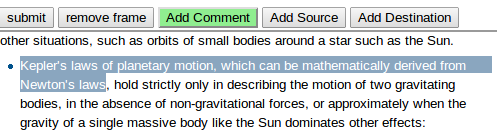
\includegraphics[width=\textwidth*4/5]{usecase/addComment.png}
				\caption{Making a selection}
			\end{figure}
			\begin{figure}[h]
				\centering
				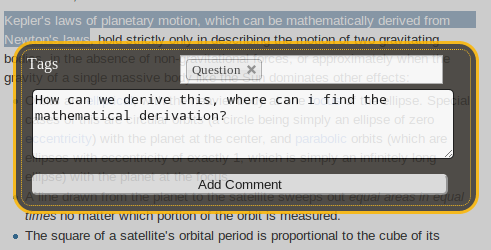
\includegraphics[width=\textwidth*4/5]{usecase/addCommentForm.png}
				\caption{Posting a comment}
			\end{figure}
			\paragraph{}
			This process of adding annotations or questions to certain parts of a web page feel very intuitive. Selecting a part of text, and writing a side note in the form fit the metaphor of highlighting a paragraph in a textbook and writing a note in the margin.
		\subsubsection*{Adding a Hyperlink} \label{sub:Adding a Hyperlink}
			\paragraph{}
			In this scenario the user does not want to ask the question about where he can find the mathematical explanation. Instead he already knows a reliable source where these calculations are explained very well. Therefore instead of adding a comment, or a note it would be much easier for the user if he could just create a hyperlink between the two documents.
			\paragraph{}
			To create the hyperlink the user needs to open a second frame by clicking the \dquote{Add Frame} button. This will split the window in two frames. Each of the frames will be able to load a different web page. In the first frame the user surfs to the web page he wanted to add the link to. In the second frame he will navigate to the web page containing the additional information that he wants the link to point to.
			\paragraph{}
			Having both these web pages open the users creates a selection on the first web page, the same way he would have done if he wanted to add a comment to the pages, as described in the previous scenario. In the second frame he will create a selection as well. This time the selection is the context of the extra information that was relevant to the selection in the first frame.
			\begin{figure}[H]
				\centering
				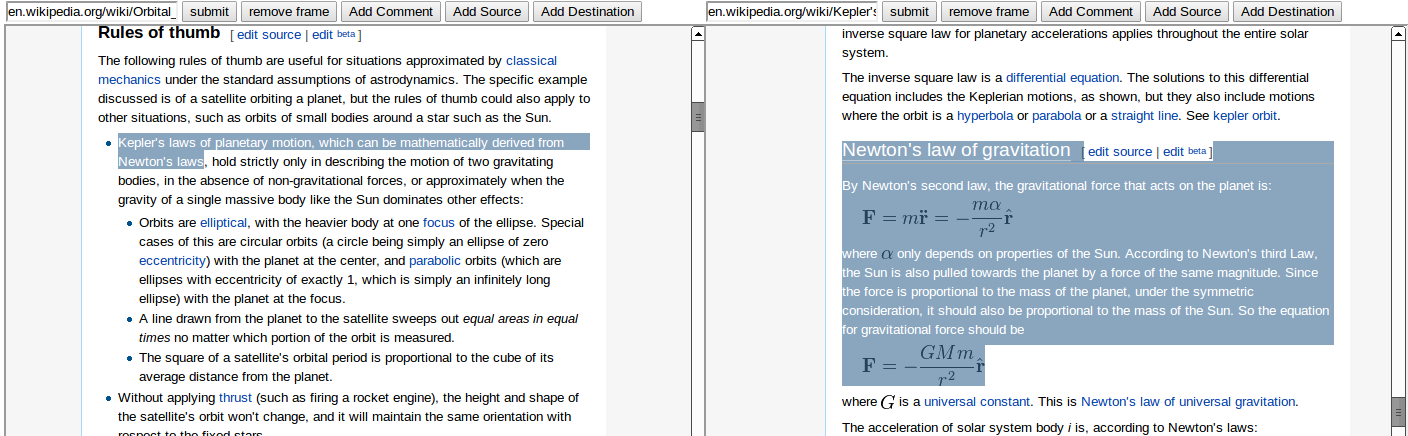
\includegraphics[width=\textwidth]{usecase/addLink.png}
				\caption{Adding a second frame with its own selection}
			\end{figure}
			\paragraph{}
			With both selections in place the user clicks the \dquote{Create Link} button in the tool bar. Clicking this button will open another pop-up window. Here the user will be presented with the option to add tags to his hyperlink and because these tags significantly help other users to find the required information the user will fill in these tags as best as possible tagging the link with \dquote{Rendezvous Manoeuvre, Mathematics, Formula}.
			\begin{figure}[h]
				\centering
				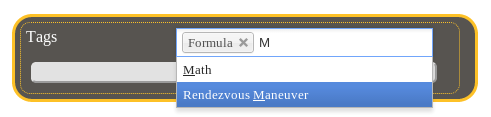
\includegraphics[width=\textwidth*4/5]{usecase/addLinkForm.png}
				\caption{Adding tags to hyperlink when the system guesses the roles}
			\end{figure}
		\subsubsection*{Multi Destination Hyperlink} \label{sub:Multi Destination Hyperlink}
			\paragraph{}
			In the previous scenario the user only linked to a single web page. Because he only had two frames open, each containing a web page the tool assumed that by clicking the \dquote{Create Link} button the user meant to create a link with one source (the left frame), and one destination (the right frame). This assumption is the intuitive approach when a user adds two documents together and therefore using \dquote{Convention Over Configuration} will speed up the process of creating these simple links.
			\paragraph{}
			In this scenario however, the link to be constructed is no longer a simple one. The user in this scenario knows about an interesting web page that describes the mathematics behind the rendezvous manoeuvre. But he also knows about a scientific paper in PDF format that explains the mathematics in far greater detail. Off course having to create two separate links for these two resources is a lot of work. So the user wants to link both of these resources to the web page in one hyperlink.
			\paragraph{}
			The process of doing so is fairly similar to the previous scenario. The difference is that the tool can no longer easily guess what frames contain the destinations, and which frame contains the source of the link. So the user will do as follows. He opens 2 additional frames in one of these frames he will navigate to the other web page he wanted to link to and in the second frame he will navigate to the PDF document. A third frame, that was already open, contains the original web page on which the link needs to be constructed.
			\paragraph{}
			With three frames open the user proceeds by specifying which frame serves what purpose. The user will click on the \dquote{Source} check mark above the third frame, specifying that the selection in this frame will be used as a source. The two other frames will be marked as destinations in the same way. With these specifications in place the user proceeds to click on the \dquote{Create Link} button and is again prompted with a similar pop-up window.
			\paragraph{}
			In this pop-up window the user can again specify the tags to describe the links. And he will do so in the same way as the previous scenario. But there is a difference here. Each destination of the link can have its own characteristics so tags can be added per destination as well. The user will do so by additionally specifying that the second destination is in fact a PDF document by adding the tag \dquote{PDF}. The three other tags are general shared tags between both destinations, while the specific \dquote{PDF} tag only applies to the second one.
			\begin{figure}[h]
				\centering
				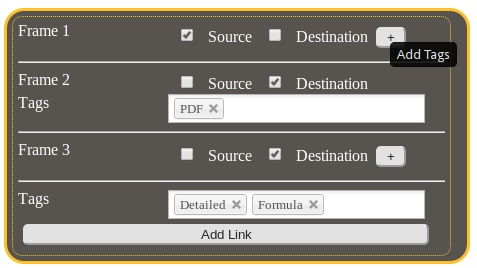
\includegraphics[width=\textwidth*4/5]{usecase/addMultiLinkForm.png}
				\caption{Manually specifying roles for selectors}
			\end{figure}
			\paragraph{}
			Any combination of many sources and many destinations can be constructed this way. The user only needs to add more selections in new frames and select the role for each of these frames.
		\subsubsection*{Multi Source On a Single Page} \label{sub:Multi Source On a Single Page}
			\paragraph{}
			In this scenario the user wants to add refer to a web page again describing the details about the mathematics behind a rendezvous manoeuvre. But instead of linking to this page from a single paragraph in on the web page he wants to link to the same web page in several separate locations in the text. A few spread out paragraphs may mention the manoeuvre but instead of providing the hyperlink only where it is mentioned first he wants to create a hyperlink on each mention of the manoeuvre.
			\paragraph{}
			The user could use the same approach as described with the previous scenario, but this would require him to open several frames displaying the same document for the sole purpose of creating several selections. This is off course cumbersome.
			\paragraph{}
			Instead the user may open two frames, the first containing the source document and the second frame containing the destination of the hyperlink. The user will then create a first selection on the first frame which represent one of the sources of the hyperlink. He will then press the \dquote{Add Source} button from the tool bar. This will temporarily save his selection and mark this selection as a source for the next creation of a hyperlink. Pressing this button will also remove the selection on that frame leaving room for a new selection.
			\begin{figure}[h]
				\centering
				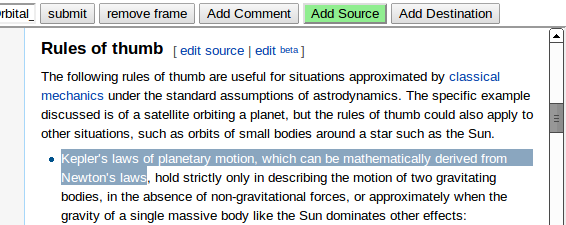
\includegraphics[width=\textwidth*4/5]{usecase/addSource.png}
			\end{figure}
			\begin{figure}[h]
				\centering
				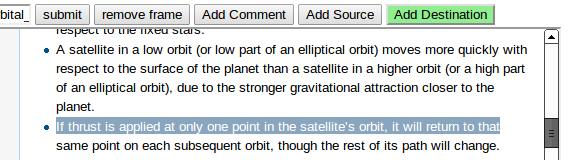
\includegraphics[width=\textwidth*4/5]{usecase/addDestination.png}
				\caption{Specify a role for an active selection}
			\end{figure}
			\paragraph{}
			After the user has selected all the locations in this document that he wants to use as a source he can do the same with any of the other frames. Marking each selection as a source or destination. When the user is done creating his selections and adding them to the appropriate roles he clicks the \dquote{Create Link} button and is presented with a familiar pop-up window prompting for more information. When the user is finished filling in the tags he will submit the form, creating the hyperlink for future users.
			\begin{figure}[h]
				\centering
				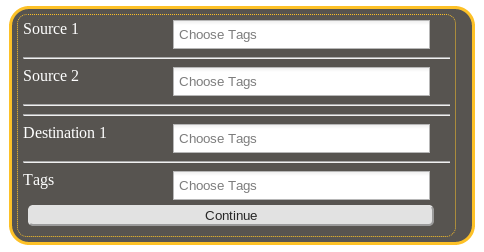
\includegraphics[width=\textwidth*4/5]{usecase/addMultiLinkManualForm.png}
				\caption{Adding tags to respective sources and destinations}
			\end{figure}
	\subsection{Navigation} \label{sub:Navigation}
	\subsubsection*{Following a Hyperlink} \label{sub:Following a Hyperlink}
		\paragraph{}
		In this scenario the user is reading the paragraph about the rendezvous manoeuvres and he wants to find more information about this topic. In order to find out if the community has already provided some hyperlinks he highlights the relevant context. This selection will update the graph view at the bottom of the screen which will now represent the metadata that is available for the selected context.
		\begin{figure}[h]
			\centering
			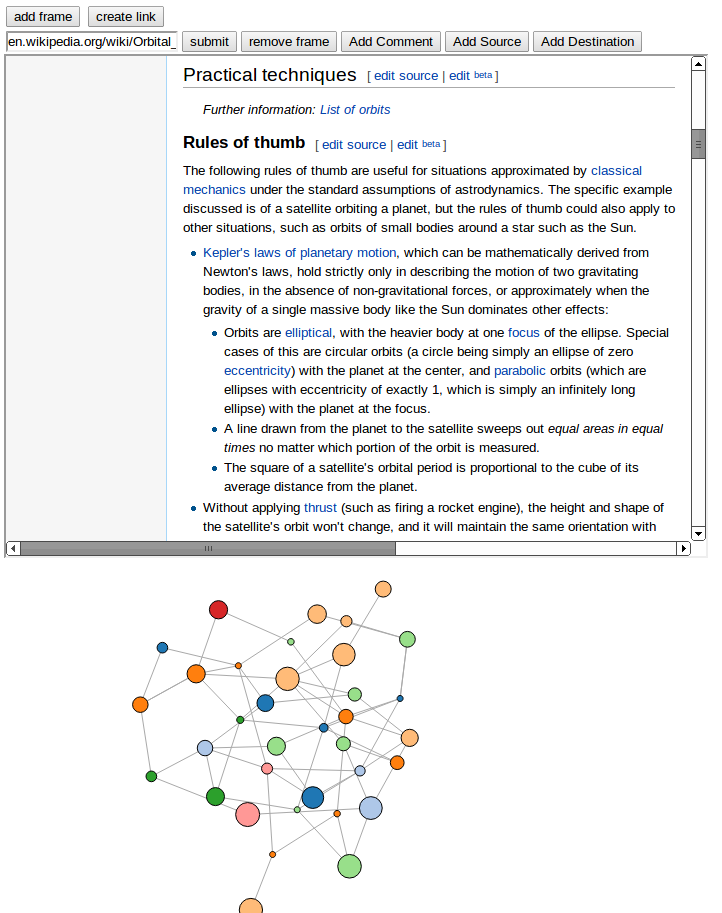
\includegraphics[width=\textwidth*4/5]{usecase/frameWithGraph.png}
			\caption{Graph and frame with no selections}
		\end{figure}
		\paragraph{}
		In this graph the user can now find all the outgoing links in his selection. Since previously other users have already added a couple of links to a web page, as well as a PDF file the user will notice this based on the colour codes of the nodes. The user is interested in the web page, so he clicks on the associated node in the graph and the tool redirects him to the appropriate web page.
		\begin{figure}[h]
			\centering
			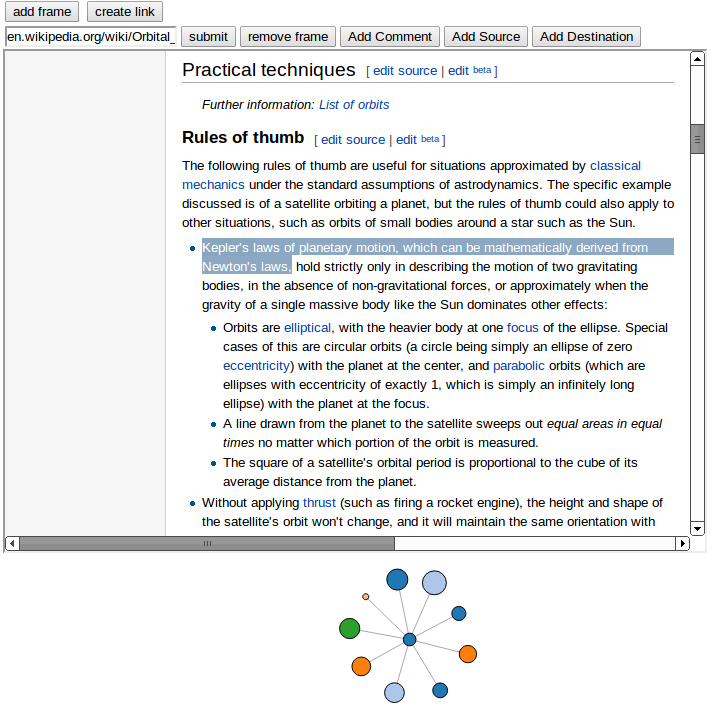
\includegraphics[width=\textwidth*4/5]{usecase/frameWithGraphSelected.png}
			\caption{Graph after making a selection}
		\end{figure}
	\subsubsection*{Searching Information} \label{ssub:Searching Information}
		\paragraph{}
		The user is faced with the same issue as the last scenario, but when he highlights the paragraph the resulting graph contains to many nodes to easily find the result he is looking for. The user is only interested in extra information about in the form of a PDF file. He also wants to find the exact mathematical formula instead of a long textual explanation about the manoeuvre. To find the intended result more quickly the users clicks in the search text field above the graph view and starts to add keywords to direct his search. The user first types the tag \dquote{PDF} but this renders far to many results to search through. Narrowing his search he will add the keyword \dquote{Formula} to the search query. Fortunately a hyperlink was added by a different user in the community containing both these tags and it is easy enough to find the requested result in the graph. Clicking on the associated node redirects the user to the requested PDF file
		\begin{figure}[h]
			\centering
			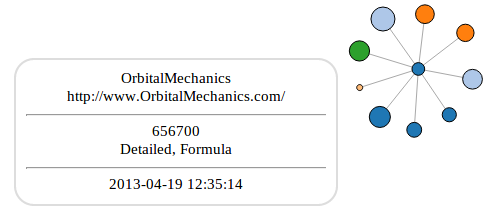
\includegraphics[width=\textwidth*4/5]{usecase/metadataGraph.png}
			\caption{Metadata on graph nodes}
		\end{figure}
	\subsection{Contribution} \label{sub:Contribution}
	\subsubsection*{Down Voting Existing Hyperlink} \label{sub:Down Voting Existing Hyperlink}
		\paragraph{}
		A user is reading the article and notices that there are two hyperlinks that point to the same resource. One of the two hyperlinks only points to a web page, while the second hyperlink points to the same web page, but also contains a PDF file as a second destination. When the user studies the extra metadata on both of the links, he notices that the tags and location of the first link are the same as the second one but the second hyperlink contains a better description as well. In short the user finds that the first hyperlink has been made obsolete by the second one. Seeing this the user wants to clear the web page of this redundant data for future users.
		\paragraph{}
		Down voting the link will help lower the popularity of the first hyperlink. Doing this will cause the redundant hyperlink to be hidden from other users. If other users will do the same eventually the obsolete metadata will be entirely removed from the web page, cleaning up the final result.
		\paragraph{}
		In order to do so the user right clicks on the node associated with the hyperlink. This will open a context menu on the node containing both the option to up or down vote the clicked hyperlink. The user then clicks on the \dquote{Down Vote} option. Doing this will send a request notifying the server of the user's contribution.
\section{Failing Scenarios} \label{sec:Failing Scenarios}
	\subsection{Blank Page} \label{sub:Blank Page}
		\paragraph{}
		In this scenario the user wants to add a simple annotation to a web page just as we described in the first scenario in the previous section. In order to do so the user opens a frame and enters the required URL in the appropriate field. But when the user submits the form nothing happens. The page stays on a black page.
		\paragraph{}
		This issue arises when a server disallows a web page to be served within a frame. The browser will notice that the \dquote{X-Frame-Option} is set in the header of the web page and will subsequently stop rendering the requested page.
		\paragraph{}
		Many large companies will not allow their website to be rendered within a frame. Companies such as Google, Facebook, Twitter, Microsoft, LinkedIn and many more will have this option set. This means that at the current state of the tool, many large and popular websites will not be able to be rendered by the tool.
	\subsection{Frame Killers} \label{sub:Frame Killers}
		\paragraph{}
		A similar situation occurs when a user wants to navigate the tool to MSN.com, Windows' live messenger website. Doing so will not yield a black page, but will in fact navigate the browser to the web page, instead of only the frame it was supposed to be loaded in. These website are running a script that, when loaded, checks whether or not the page was loaded in a frame. In the case of our tool this check will detect this and point the browser to the website instead of the frame. These frame killers, as they are called, will refresh the page which leads to a removal of the tool bars our tool provided. Therefore on these type of websites the users will not be able to add hyperlinks or comments.
	\subsection{Dynamic Pages} \label{sub:Result Mismatech}
		\paragraph{}
		In this example the user wants to add a link to a particular paragraph in an interesting blog posts. He will again select the source in the first frame, and the destination in the second frame, containing the blog. Clicking the \dquote{Create Link} button will finish the process and everything is in order. Users visiting the page will see the link, and following the link will direct them to the intended blog post.
		\paragraph{}
		However, a couple days later a users tries to follow the hyperlink and is redirected to the blog website. But the posts the user sees are not relevant to the context in which the link appeared. And in fact he can not see the destination of the link at all.
		\paragraph{}
		This effect is because of the way blog websites usually work. When the blogger adds a new post to his website the newest item will appear at the top, pushing all older items down. When to many items are on the front page the rest of the posts are paginated and require the reader to click on a link to see them. This behaviour is fairly standard but it poses a problem for the tool.
		\paragraph{}
		When a hyperlink is created the metadata for this link contains pointers to different resources, the sources of the hyperlink and the destinations. These resources can be PDF files, websites, video or audio files, and many more different types of media. In this case both the source and destination of the hyperlink are websites. The identifier of this resource is defined by its URL. So when the user links to the blog website he will create a pointer that points to a specific location in the resource that is identified by the specified URL. Lets say the destination of the hyperlink was a sentence in the first post of the website \dquote{www.blog.com}.
		\paragraph{}
		So on creation the hyperlink will work fine and point to the first post on the web page which, at the time, contained relevant information. After a while the owner of the blog will post new articles which will most likely not be related to the link's intended topic. Because of the restructuring of the web page the destination pointer of the hyperlink will no longer be valid. This will mislead or confuse visitors following the hyperlinks.
		\paragraph{}
		In Section \ref{sub:Workarounds} \nameref{sub:Workarounds} we already discussed some methods of helping with this problem but they are not infallible and the scenario we just described can still take place.
%	\subsection{Delayed Content} \label{sub:Delayed Content}
	
\section{Conclusion} \label{sec:Conclusion}
	\paragraph{}
	In this chapter, we have demonstrated some of the usages of our tool by means of some simple scenarios. As one can see many of the features are intuitive and simple to use providing an easy way of creating advanced links between different media. The functionality demonstrated by these simple examples represent only the beginning of the potential of the tool. When more visualisations are designed more features will be available for the user resulting in a richer user experience.
	\paragraph{}
	It is also important to note that many of the failing examples stem from restrictions in the current web standards. Security issues that plagued the web have resulted in a strict security protocol which dampens a lot of possibilities. And creating a more persistent way of selecting a part of a document will result in more robust linking overall.

%!TEX root = thesis.tex 

\chapter{Conclusions and Future Work} \label{cha:Conclusions and Future Work}
\paragraph{}
In this final chapter, we would like to recapitulate a number of contributions that have been made. As we were limited by the time constraint of this thesis, some  envisioned features were not yet implemented. Therefore we will outline and discuss some future directions for our linking tool.

\section{Contributions} \label{sec:Contributions}
\paragraph{}
The literature study that has been carried out as part of this thesis shows that there is room for improvements in the area of hyperlinking on the Web. The market of web browsers is heavily dominated by classic browsers such as Internet Explorer, Google Chrome and Firefox and these browsers have heavily influenced the Web's linking standard.
\paragraph{}
While there are alternative approaches available, these tools often specialise on specific features instead of the linking process as a whole. Many of these tools also neglect the upcoming trend of sharing user created data. Nevertheless, by studying these tools, we learned a few valuable lessons concerning the ways of enhancing the Web's linking experience and how they relate to the limitations of the current web standard.
\paragraph{}
By combining the different aspects that we deem beneficial for our tool with our own ideas for an ideal tool, we came up with a model and architecture for an advanced linking tool addressing many of the issues the current state-of-the-art hyperlinking tools. Our tool steps away from the classic restrictions of the two dimensional web page and is based on state-of-the-art research from fields such as hypermedia, zoomable user interfaces and data visualisation in order to redesign the way we use hyperlinks on the Web.
\paragraph{}
Our investigation of the state-of-the-art in hypermedia, data visualisation and zoomable user interfaces helped us to avoid some of the pitfalls when designing out tool. What follows is a description of the steps we took, and contributions we made during this thesis
\begin{itemize}
	\item A literature study has been done in order to identify issues with current linking tools. We compared the benefits of state-of-the-art linking tools to the standard HTML approach in order to use our findings in our work.
	\item Based on our findings from the literature study and a closer investigation of existing tools, we identified technologies that might be beneficial in the creation of an advanced hyperlinking tool and help us to overcome some of the limitations these tools suffer. Based on this analysis we listed the benefits and drawbacks of a large amount of options we have for our tool and based on this list we created a design for our ideal linking tool. After careful deliberation regarding the use of concepts and technologies, we provided a solution that mitigates or eliminates many of the issues and shortcomings with existing tools.
	\item Based on our analysis of the limitations of state-of-the-art web linking tools we created a set of requirements for our tool and we defined a model and architecture for our proposed solution.
	\item Finally we implemented a functional prototype of our tool which uses many of the innovative features and forms the basis of our advanced hyperlinking tool.
\end{itemize}
Because of our requirement to build the tool using JavaScript only, we opted to build the tool from scratch. This allowed us to leave conventional approaches behind. Doing so allowed us to keep in mind the core requirements when building the foundations of the tool which inevitably leads to a better designed tool that provides to most functionality and extensibility.
\section{Future Work} \label{sec:Future Work}
\paragraph{}
Because of the limited time available for this thesis,  some extensions and features did not make it to the final implementation, thus the tool has not yet reached its full potential. Therefore we made sure that we finished a solid foundation on which future features can be implemented. We did not rush the implementation in favour of excessive features and different visualisations, instead we opted to ensure that we got the basics right and modular from the beginning so that extensions are easily implemented. As a result we did not have time left to implement many different visualisations which would emphasise the power of our tool. In this section, we discuss some extensions and future work that will help bring our tool a step closer to its full potential.
\section{Robustness} \label{sec:Robustness}
\paragraph{}
One of the big limitations of our tool is the suboptimal performance on highly dynamic web pages. When the content of the web page changes while the page's identifier stays the same, it is possible that the selectors of previously saved hyperlinks will have a mismatch on the content of the page. This will of course break existing links, should the content of the web page change, but it also makes the tool not viable on websites with highly dynamic pages such as most of the Google web services. Detecting whether the content of the web page has changed since the time the hyperlink was created can be done by hashing the web page when the hyperlink is created and then matching this hash with the hash of the current content on the page. When the hashes do not match we have detected that the content has changed.
\paragraph{}
One way to minimise the amount of breaking hyperlinks is by detecting whether the content on which the hyperlink was created is still available. The content of the web page might have moved around a bit in such a way that the XPointer of the related selector is no longer valid, but the content is still there. If we can detect this, many hyperlinks that would otherwise break, can still be valid. Imagine a blogging website where each new post is listed at the top, moving all previous post down on the page. Hyperlinks created on any of these blog posts would break every time a new post was created with the current method, but if we check the content of the web page, these hyperlinks will be valid for a substantially longer period of time.
\section{Interactivity} \label{sec:Interactivity}
\paragraph{}
We are aware that we did not yet devote a lot of attention to editing and removing existing hyperlinks or selectors which would lead to more technical problems when the database grows. We have already implemented a means of detecting when hyperlinks are no longer deemed interesting by the community and this metric can be used to automatically remove hyperlinks from the database. But when the users make a mistake and want to edit or remove their hyperlinks they are currently unable to do so.
\paragraph{}
We are currently heavily reliant on the users' capability to create a selection on a web page, but on many new devices this is not necessarily straightforward or easy. Many smartphones or tablets do not allow users to easily create selections in their web browsers, which limits the tools usefulness on these devices. With better interactive possibilities to create selectors, the tool could be used on more devices and by more users.
\paragraph{}
When new filters and visualisations get introduced this will bring the need to manipulate these visualisations as well, introducing the need for more advanced interactivity.
\section{Visualisation} \label{sec:Visualisation}
\paragraph{}
The biggest trump of our tool is the versatility with which the metadata can be visualised. Many diverse questions can be easily answered with different visualisations and for a further extension of the tool many new interesting and useful ways of data visualisation can be added. Because of our limited time we only opted to implement some of the more obvious visualisations but many unused dimensions of the metadata can still be presented to the users in such a way that the information is easy accessible.
\section{General} \label{sec:General}
\paragraph{}
As we can see, most of the work carried out in this thesis covers the foundation of an extendible tool for advanced hyperlinking. In future work, additional research could be done for more diverse visualisations and interactions. Additional research regarding the filtering techniques can also increase the effectiveness of the tool and by extension the usefulness for the end users. Finally, including additional media types and the support for transclusion, will elevate the tool to a true collaborative cross-media hyperlinking tool that scales well with the amount of users.
\paragraph{}
Even though we were able to identify the many shortcomings of current state-of-the art hyperlinking tools, propose innovative features for non-restricted hyperlink visualisation and provide a prototype implementation of a next generation hyperlinking tool, our tool has to be seen as the foundation of an extendible collaborative hyperlinking solution.


%
% BIBLIOGRAPHY
%

\newpage
\bibliographystyle{abbrv}
\bibliography{bibliography}

\end{document}
